\documentclass[letterpaper,journal]{IEEEtran}
\usepackage[T1]{fontenc}
\usepackage{amsmath,amsfonts}
\usepackage{algorithmic}
\usepackage{algorithm}
\usepackage{array}
\usepackage[caption=false,font=footnotesize,labelfont=sf,textfont=sf]{subfig}
\usepackage{textcomp}
\usepackage{stfloats}
\usepackage{url}
\def\UrlBreaks{\do\/\do\-\do\_}
\usepackage{verbatim}
\usepackage{graphicx}
\usepackage{cite}
\usepackage{multirow}
\usepackage{balance}
\usepackage{placeins}
\hyphenation{op-tical net-works semi-conduc-tor IEEE-Xplore}

\begin{document}

\title{MultiEMiT: Multimodal Emotion, Irony, and Semiotic Relation Detection in Italian Social TV}

\author{Author~Author,~\IEEEmembership{Graduate Student Member,~IEEE,}
        Co-Author~One,~\IEEEmembership{Member,~IEEE,}
        and~Co-Author~Two,~\IEEEmembership{Senior Member,~IEEE}%
\thanks{TODO}%
\thanks{TODO}}

% The paper headers
\markboth{IEEE Transactions on Affective Computing,~Vol.~XX, No.~X, October~2026}%
{Author \MakeLowercase{\textit{et al.}}: MultiEMiT: Multimodal Affective Computing in Italian Social TV}

\maketitle

\begin{abstract}
During live television broadcasts, viewers frequently share comments, screenshots, and memes on social media to express their opinions and reactions. Analyzing affective intent in this setting is challenging because posts are brief, informal, and inherently multimodal. Accompanying images do not simply repeat the text; they often add context, amplify tone, or completely change the literal meaning. In this paper, we introduce MultiEMiT, a multimodal dataset of Italian Social TV commentary annotated across five pragmatic layers: Plutchik's fine-grained emotions, irony and sarcasm, offensiveness, target orientation (program format versus broadcast topic), and semiotic text--image relations. We evaluate both compact Dual-Encoder models and a large generative vision--language model (Pixtral 12B). To explore how much information is shared across tasks, we also study correlation prompting, where labels from auxiliary annotation layers are added to the input text. Our findings reveal that visual context plays very different roles across tasks. For irony detection, images provide a direct and significant improvement, as irony often stems from the contrast between text and image. In contrast, for emotion recognition, images alone yield little benefit, helping only when combined with auxiliary task labels. For semiotic relation detection, concatenating text and image features fails to beat text baselines, whereas fine-tuning Pixtral achieves the highest score despite struggling with minority classes. MultiEMiT provides both a new resource and an exploratory benchmark for understanding how multimodal models handle complex, real-world social commentary.
\end{abstract}

\begin{IEEEkeywords}
Affective computing, multimodal emotion recognition, irony detection, vision-language models, Social TV.
\end{IEEEkeywords}

\section{Introduction}
\IEEEPARstart{T}{elevision} audiences no longer watch broadcasts in silence. During live debates, political talk shows, and reality competitions, viewers actively turn to second-screen platforms like Twitter to share commentary, memes, and screenshots \cite{SocialTV}. This stream of real-time viewer feedback offers broadcasters far richer signals than traditional audience ratings, providing immediate insight into public controversy, approval, and emotional engagement \cite{memorai}. 

Capturing these affective signals computationally, however, presents severe challenges. Social TV commentary is short, colloquial, and inherently multimodal. Viewers attach screengrabs and reaction images that do not merely mirror the written text; they exaggerate emotional tone, introduce sarcasm, or invert the literal message completely \cite{schifanella2016multimodal, cai2019multimodal}. 

The foundational question that motivated this investigation is: \textit{how much do attached images genuinely contribute to identifying human affective intent in multimodal social network posts?} \cite{poria2017review} During the manual annotation of our dataset, we observed a crucial empirical phenomenon: human annotator agreement increased substantially when annotators were provided with the attached images compared to reading the text alone. Visual context anchored ambiguous social commentary, establishing consensus where text alone yielded divergent interpretations. This observation directly motivates our central research hypothesis: \textit{does this visual grounding similarly carry over to neural models, and does it hold equally for literal and figurative discourse?}

Furthermore, while multilingual initiatives have advanced text-based emotion analysis, computational resources for Italian remain scarce, and existing benchmarks focus exclusively on unimodal text \cite{bianchi2021feel, emit, MultiEmotion}. To bridge this gap, we introduce \textbf{MultiEMiT}, a multimodal dataset of Italian Twitter commentary gathered from television broadcasts. MultiEMiT provides annotations across five pragmatic layers: fine-grained emotions under Plutchik's taxonomy \cite{Plutchik}, irony and sarcasm, offensiveness, target orientation (program container versus broadcast content), and semiotic text-image relationships \cite{MultiM}. Our benchmarking focuses on three primary classification tasks: Emotion Detection, Irony Detection, and Semiotic Relation Detection, with offensiveness and target serving as contextual signals. To expand training coverage for baseline text encoders, we also draw on the external unimodal EMiT (for Emotions) \cite{emit} and IronITA (for Irony) \cite{ironita2018} corpora.

An in-depth statistical analysis of MultiEMiT's multi-layered annotations revealed another compelling pattern: extensive empirical co-occurrences connect different annotation levels. For instance, irony correlates with joy, sarcasm pairs strongly with disgust and offensiveness, and program-directed commentary associates with viewer trust. Rather than treating these dimensions as isolated tasks, we investigated how much information each annotation layer carries about the others. To this end, we propose \textbf{Correlation Prompting}, a strategy that exposes the remaining annotation layers to the model in natural language: trained encoders receive verbalized auxiliary annotations prepended to each post and learn their association with the target labels, while generative models used without task-specific training additionally receive the corpus-level Pearson correlation rules in their instructions. Since gold auxiliary labels are supplied at inference time, this setting serves as an oracle probe of the informativeness of each annotation layer rather than as a deployable system.

Since our goal is to characterize the resource and its possibilities rather than to maximize performance, we frame our study around three core research questions:
\begin{itemize}
    \item \textbf{RQ1 (Visual Context):} Does adding visual context help neural models detect emotion, irony, and semiotic relations, and does its contribution differ across tasks?
    \item \textbf{RQ2 (Correlation Prompting):} Does exposing the auxiliary annotation layers in the model input improve classification across discriminative and generative architectures?
    \item \textbf{RQ3 (Architectural Paradigms):} How do compact discriminative models (BERT-ViT Dual-Encoders with linear classifiers on frozen features) compare with a 12 billion parameter vision--language model (Pixtral 12B) on a shared test set?
\end{itemize}

The main contributions of this work are summarized as follows:
\begin{itemize}
    \item We introduce \textbf{MultiEMiT}, the first multimodal dataset of Italian Social TV commentary, annotated across five pragmatic layers and validated through three-annotator adjudication.
    \item We show that the role of visual context depends strongly on the task: images directly help irony detection by capturing text--image contrast, but help emotion recognition only when combined with auxiliary task labels.
    \item We analyze \textbf{Correlation Prompting} as an exploratory method to examine how much information is shared across annotation layers, testing how auxiliary labels guide both traditional classifiers and generative models.
    \item We compare compact Dual-Encoder baselines with the 12B parameter Pixtral model on a shared test set, highlighting differences in how they handle class imbalance and complex semiotic relations.
\end{itemize}

The rest of this paper is organized as follows. Section~\ref{sec:related_works} situates MultiEMiT within Italian affective computing, Social TV analytics, and multimodal document intent. Section~\ref{sec:dataset_analysis} describes the corpus collection, annotation protocol, and cross-dimensional correlations. Section~\ref{sec:experimental_design} defines our classification tasks, Dual-Encoder architecture, correlation prompting strategy, and Pixtral configurations. Section~\ref{sec:results} presents comparative evaluations and subset analyses across semiotic relations. Section~\ref{sec:conclusion} summarizes our findings and directions for future work.
\section{Related Work}
\label{sec:related_works}

As affective computing shifts from sentiment polarity \cite{SOMSA} toward discrete emotion recognition, recent large scale initiatives like BRIGHTER \cite{brighter_project} highlight a persistent scarcity of native, language specific datasets. Because emotional expression is deeply contextual and shaped by cultural and linguistic norms, translated resources fail to capture fine-grained taxonomies such as Plutchik's Wheel of Emotions \cite{Plutchik, mohammad2018semeval}. While Italian is represented by foundational text corpora like FEEL-IT \cite{bianchi2021feel}, resolving the ambiguity of Plutchik's eight emotion schema in highly contextual domains, such as social media commentary on television broadcasts, remains a complex challenge. To address these nuances, we introduce \textit{MultiEMiT}, the first Italian multimodal dataset featuring multi-level annotations designed to capture both textual and visual emotional cues.

Early Italian resources focused strictly on binary or three class polarity \cite{barbieri2016sentipolc}. The first dedicated shift toward fine-grained categories came with \textit{FEEL-IT} \cite{bianchi2021feel}, which collected 2,037 tweets across politics, sports, and healthcare during 2020. Annotated with a subset of four basic emotions from Ekman's model \cite{ekman1992argument} (anger, joy, sadness, fear), FEEL-IT established that Italian language models like UmBERTo \cite{musixmatch-2020-umberto} produce reliable affective classifiers. Yet a four class schema misses mixed feelings and conversational nuances common in viewer reactions. To address broader emotional ranges, \textit{MultiEmotions-It} \cite{MultiEmotion} annotated YouTube and Facebook comments across Plutchik's eight primary emotions \cite{Plutchik}, polarity, and sarcasm. Their findings showed that while polarity models perform consistently, multi-label emotion recognition and sarcasm detection suffer from severe class sparsity and label ambiguity.

Second screen platforms have changed how broadcasters analyze viewer engagement \cite{SocialTV}. Traditional television ratings measure raw viewer counts; they cannot infer whether an audience is laughing, outraged, or sympathetic. The \textit{M.EMO.RAI} project was formed to address this limitation, establishing a joint partnership between the University of Turin and Rai (Radiotelevisione Italiana) \cite{memorai}. The goal was an automated system to track audience reactions during live broadcasts by ingesting public social network commentary.

This partnership led to the \textit{EMiT} (Emotions in Italian) corpus, benchmarked as an EVALITA 2023 shared task \cite{emit}. With 5,966 social media posts from live broadcasts (including the Sanremo Festival and scripted drama), EMiT adopted Plutchik's taxonomy. It also introduced the \textit{Target} dimension, distinguishing whether a comment attacks the broadcast \textit{Content} (the topic, guest, or political issue) or evaluates the \textit{Container} (the host, studio format, or network production). EVALITA benchmark results showed that while classifiers perform well on familiar shows, accuracy drops on out-of-domain broadcasts. To expand training coverage and alleviate class sparsity on long-tail categories, we use external EMiT data in a domain warm-up step when fine-tuning our emotion encoders, while evaluating strictly on held-out MultiEMiT test instances.

Irony detection requires models to recognize when a speaker's intended meaning opposes their literal words. In Italian NLP, the standard benchmark is \textit{IronITA} \cite{ironita2018}, curated for EVALITA 2018 with nearly 5,000 tweets annotated for irony and sarcasm (defined as hostile or denigratory mockery). Results on IronITA showed that text-only classifiers struggle on short posts when pragmatic context is missing. To provide our models with broader training coverage on figurative language, we use the external IronITA dataset in a domain warm-up step when fine-tuning our UmBERTo irony encoders, while evaluating strictly on MultiEMiT test splits.

Linguistic text only tells half the story in modern social media. In their study on multimodal document intent, Kruk et al. \cite{MultiM} demonstrated that images in social posts rarely just illustrate captions; rather, they alter communicative intent through three distinct semiotic relationships: \textit{parallel}, where image and text independently convey the same underlying meaning; \textit{additive}, where the two modalities amplify or modify one another; and \textit{divergent}, where visual and textual cues pull in opposite directions to create a semantic gap. Incongruent or divergent pairings are particularly critical in social media, as they frequently generate memes, irony, and satirical humor by subverting the literal text \cite{schifanella2016multimodal, cai2019multimodal}. Related studies on Twitter have similarly categorized how visual media expands or redirects short textual posts \cite{vempala2019categorizing}; however, these studies focused exclusively on English posts, leaving the interplay between text and visual media in Italian television commentary largely unexplored. \textit{MultiEMiT} addresses this gap by applying this semiotic framework directly to Italian Social TV.
\section{Dataset Analysis}
\label{sec:dataset_analysis}

We introduce the MultiEMiT corpus, a multi-layered multimodal dataset of Italian Twitter commentary gathered during live television broadcasts. The data originates from the M.EMO.RAI project \cite{memorai}, which set out to track audience emotional responses in real time. Rather than restricting annotations to positive or negative sentiment, MultiEMiT applies an expanded eight-emotion taxonomy derived from Plutchik's psychoevolutionary model \cite{Plutchik}.

MultiEMiT was collected from two television broadcasts, representing contrasting formats and registers:

\textit{ProSAT:} Twitter commentary on \textit{Propaganda Live}, a satirical talk show on LA7 combining investigative journalism and political commentary \cite{propagandalive}. The collection captures the broadcast of November 19, 2021, when host Diego Bianchi reported live from the Poland-Belarus border during a humanitarian crisis. The gravity of the event prompted solemn reactions dominated by indignation, grief, and civic debate.

\textit{EMiT (Pechino Express):} Inspired by the EVALITA 2023 EMiT benchmark \cite{emit}, this sub-corpus covers \textit{Pechino Express}, an adventure reality show broadcast on Rai2 \cite{pechinoexpress}. Collected during the season premiere on February 11, 2020, viewer discourse centers on lighthearted entertainment, contestant rivalries, and humorous commentary.

Both collections share an identical structure: a purely textual partition and a multimodal partition pairing the text with its attached media (screenshots, edited images, and memes). This paired structure allows direct comparison between unimodal and multimodal models, showing where visual content modulates the written post. In addition to MultiEMiT, two external Italian textual corpora are used as supplementary training data only: EVALITA 2023 EMiT (5,966 posts across multiple programs \cite{emit}) for emotion detection and IronITA (4,849 posts \cite{ironita2018}) for irony detection.

Annotation was conducted on Sensitag, a web annotation platform developed at the University of Turin. Each post was evaluated independently by three annotators with backgrounds in computer science or linguistics. Final labels were assigned by majority vote (at least two out of three annotators agreeing) to create a golden dataset.

\begin{figure}[!t]
\centering
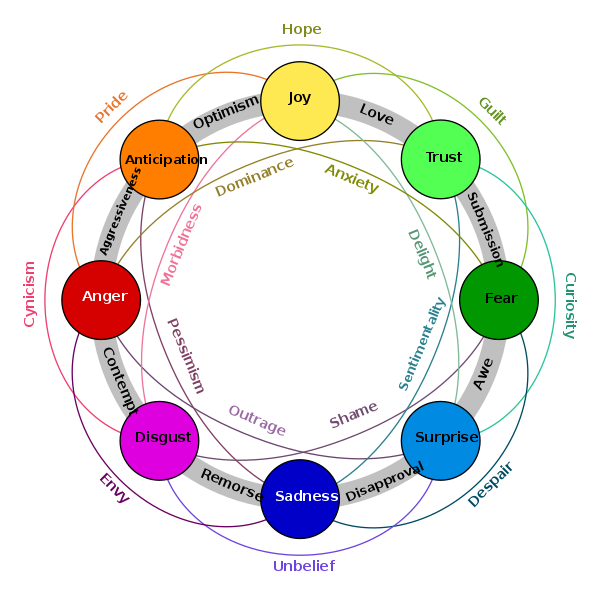
\includegraphics[width=0.88\columnwidth]{imgs/Plutchik_Dyads.svg.png}
\caption{Robert Plutchik's psychoevolutionary emotion schema \cite{Plutchik} and derived affective dyads. Primary emotional axes arranged along the perimeter combine systematically into secondary and tertiary affective blends (e.g., \textit{Joy} + \textit{Trust} yields \textit{Love}, while \textit{Disgust} + \textit{Anger} yields \textit{Contempt}).}
\label{fig:plutchik_dyads}
\end{figure}

The corpus is annotated across five pragmatic dimensions:
\begin{itemize}
    \item \textbf{Emotions:} Ten affective categories grounded in Plutchik's psychoevolutionary model \cite{Plutchik} (\textit{Joy}--\textit{Sadness}, \textit{Trust}--\textit{Disgust}, \textit{Fear}--\textit{Anger}, \textit{Surprise}--\textit{Anticipation}), supplemented with \textit{Love} and \textit{Neutral}. According to Plutchik's theory, primary emotional axes combine systematically along the wheel into complex secondary and tertiary affective states, termed \textit{dyads} (e.g., \textit{Trust} + \textit{Joy} = \textit{Love}, \textit{Disgust} + \textit{Anger} = \textit{Contempt}, \textit{Sadness} + \textit{Disgust} = \textit{Remorse}, or \textit{Anger} + \textit{Surprise} = \textit{Outrage}), as illustrated in Fig.~\ref{fig:plutchik_dyads}. This combinatory nature provides theoretical justification for formulating emotion detection as a multi-label task \cite{mohammad2018semeval, demszky2020goemotions}, allowing social media posts to express complex or multiple emotions.
    \item \textbf{Irony and Sarcasm:} Three exclusive classes separating literal statements (\textit{Unironic}), humorous figurative inversion (\textit{Irony}), and hostile, denigratory mockery (\textit{Sarcasm}).
    \item \textbf{Offensiveness:} A binary indicator identifying abusive language, insults, or harassment directed at individuals or protected groups (incorporating rare hate speech instances due to their scarcity in broadcast commentary; all remaining posts are non-offensive).
    \item \textbf{Target:} Distinguishes whether comments address the broadcast \textit{Content} (political issues, guests, or news events) or the \textit{Container} (the studio host, network, or production execution). Because posts may use the broadcast hashtag without referencing the program itself, or comment on both aspects at once, a post can have no target (292 textual and 58 multimodal posts) or both targets simultaneously (61 textual and 7 multimodal posts).
    \item \textbf{Semiotic Relation:} Categorizes multimodal document intent based on the semiotic taxonomy established by Kruk et al. \cite{MultiM} into three foundational relationships (depicted in Fig.~\ref{fig:semiotic_relations}): \textit{Additive}, where text and image mutually enrich and expand each other to produce a cohesive narrative; \textit{Parallel}, where both text and visual media redundantly express the same semantic information independently; and \textit{Divergent}, where textual and visual cues convey contrasting or incongruent signals, creating cognitive dissonance, ironic tension, or meme subversion.
\end{itemize}

\begin{figure*}[!t]
\centering
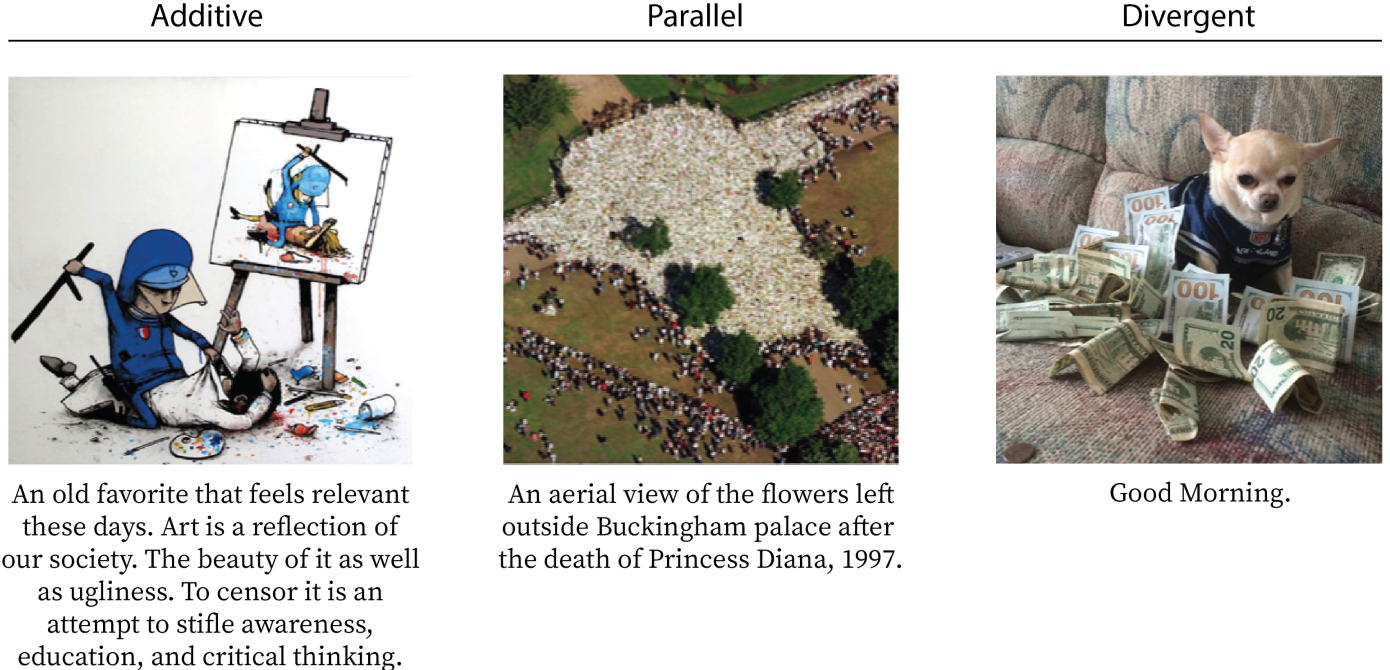
\includegraphics[width=0.92\textwidth]{imgs/Additive_divergent_parallel.png}
\caption{Taxonomy of semiotic text--image relationships defined by Kruk et al. \cite{MultiM}: \textit{Additive} (text and image mutually enrich one another to produce new contextual depth), \textit{Parallel} (both modalities independently deliver redundant semantic meaning), and \textit{Divergent} (semantic or pragmatic conflict between modalities, generating irony, cognitive tension, or satirical contrast).}
\label{fig:semiotic_relations}
\end{figure*}

\begin{figure}[!t]
\centering

\includegraphics[width=0.95\columnwidth]{imgs/interpretation_of_posts.png}
\caption{Example of an ambiguous Social TV post from the \textit{Propaganda Live} collection evaluated by three independent annotators. Despite viewing identical multimodal content, each annotator assigned a distinct emotional reading (\textit{Anger}+\textit{Disgust} vs. \textit{Sadness}+\textit{Surprise} vs. \textit{Disgust}+\textit{Fear}), illustrating the inherent difficulty of human agreement in subjective affective tasks and the pruning effect of majority-voting gold standard consolidation.}
\label{fig:interpretation_of_posts}
\end{figure}

Emotions in short social media commentary are inherently ambiguous, and human annotators frequently diverge in their subjective interpretations. Figure~\ref{fig:interpretation_of_posts} illustrates a compelling example from the \textit{Propaganda Live} collection, where the post \textit{``Terrible, I'm ashamed of being European''} was paired with broadcast stills of shivering refugee families at the Poland--Belarus border. Despite reading the exact same text and inspecting the same imagery, the three independent annotators arrived at three distinct emotional interpretations:
\begin{itemize}
    \item \textit{Annotator 1} marked \textit{Anger} and \textit{Disgust}, interpreting the post as indignant moral outrage toward European governance;
    \item \textit{Annotator 2} selected \textit{Sadness} and \textit{Surprise}, reading it as shocked disbelief and disapproval;
    \item \textit{Annotator 3} chose \textit{Disgust} and \textit{Fear}, capturing internalized shame and apprehension.
\end{itemize}
Under our strict majority-voting protocol (which requires agreement from at least two out of three annotators to retain a label in the golden dataset), only the overlapping label \textit{Disgust} was preserved, while the distinct yet plausible secondary interpretations were pruned. This example vividly underscores the challenge of achieving human annotator consensus on subjective social media tasks \cite{demszky2020goemotions, basile2021disagreement}.

\begin{table}[!t]
\centering
\caption{Inter-Annotator Agreement (Fleiss' $\kappa$) across Pragmatic Dimensions and Multimodal Disambiguation Gain on Paired Posts ($N = 628$)}
\label{table:fleiss_kappa}
\footnotesize
\setlength{\tabcolsep}{2.5pt}
\renewcommand{\arraystretch}{1.05}
\resizebox{\columnwidth}{!}{%
\begin{tabular}{l | c c | r}
\hline
\textbf{Pragmatic Dimension} & \textbf{Text-Only} & \textbf{With Image} & \textbf{Visual Gain} \\
\textbf{/ Category} & \multicolumn{2}{c|}{\textbf{(Paired $N = 628$)}} & \textbf{($\Delta\kappa$ / \%)} \\
\hline
\multicolumn{4}{l}{\textit{Emotions (Plutchik)}} \\
\hline
Love & 0.270 & 0.159 & $-0.111$ ($-41.2$\%) \\
Anticipation & 0.469 & 0.573 & +0.104 (+22.3\%) \\
Disgust & 0.518 & 0.522 & +0.005 (+0.9\%) \\
Trust & 0.444 & 0.515 & +0.072 (+16.1\%) \\
Joy & 0.451 & 0.390 & $-0.062$ ($-13.7$\%) \\
Fear & 0.172 & 0.215 & +0.043 (+24.7\%) \\
Anger & 0.353 & 0.454 & +0.101 (+28.5\%) \\
Surprise & 0.246 & 0.255 & +0.009 (+3.7\%) \\
Sadness & 0.272 & 0.312 & +0.039 (+14.5\%) \\
Neutral & 0.274 & 0.359 & +0.085 (+31.0\%) \\
\hline
\textbf{Emotion Level Mean} & \textbf{0.347} & \textbf{0.375} & \textbf{+0.028 (+8.2\%)} \\
\hline
\multicolumn{4}{l}{\textit{Irony and Sarcasm}} \\
\hline
Irony & 0.426 & 0.596 & \textbf{+0.171 (+40.0\%)} \\
Sarcasm & 0.302 & 0.319 & +0.018 (+5.9\%) \\
\hline
\multicolumn{4}{l}{\textit{Target}} \\
\hline
Container & 0.512 & 0.546 & +0.034 (+6.6\%) \\
Content & 0.474 & 0.657 & \textbf{+0.183 (+38.6\%)} \\
\hline
\multicolumn{4}{l}{\textit{Offensiveness}} \\
\hline
Offensive / Hate Speech & 0.370 & 0.549 & \textbf{+0.179 (+48.6\%)} \\
\hline
\multicolumn{4}{l}{\textit{Semiotic Relation}} \\
\hline
Additive & -- & 0.461 & -- \\
Divergent & -- & 0.675 & -- \\
Parallel & -- & 0.364 & -- \\
\hline
\textbf{Cumulative Schema Gain} & \textbf{5.553} & \textbf{6.422} & \textbf{+0.869 (+15.6\%)} \\
\hline
\end{tabular}%
}
\end{table}

At the same time, providing annotators with the accompanying visual media systematically resolved human interpretive ambiguity. Table~\ref{table:fleiss_kappa} details Inter-Annotator Agreement (Fleiss' $\kappa$) across all five pragmatic dimensions for the controlled paired evaluation on the multimodal subset ($N = 628$) annotated independently both with and without visual attachments. Of the 645 multimodal posts in the consolidated corpus, 628 possess complete three-annotator triads across both with-image and text-only control conditions and constitute the paired disambiguation sample for Table~\ref{table:fleiss_kappa}; the remaining 17 posts were labeled by two raters in the raw logs and are retained in the gold-standard benchmark splits for machine learning. Access to visual context produces a consistent agreement boost across the entire pragmatic schema ($+15.6\%$ cumulative gain), demonstrating that images anchor viewer interpretation.

This disambiguating effect is particularly striking on pragmatic and figurative layers that rely on contextual grounding. On \textit{Offensiveness} and \textit{Irony}, agreement surges by over 40\%, as visual cues readily distinguish genuine hostility from playful banter and reveal figurative inversions that remain imperceptible in isolated text. Similarly, visual context clarifies whether commentary targets the broadcast's political \textit{Content} or production \textit{Container}. Within the affective spectrum, images sharpen consensus around indignant reactions (\textit{Anger} and \textit{Anticipation}), while slightly reducing surface agreement on \textit{Love} and \textit{Joy}---an effect driven by sarcastic memes whose visual incongruity exposes biting satire masked behind superficially positive words. Finally, annotators achieve substantial agreement on \textit{Divergent} semiotic relations ($\kappa = 0.675$), confirming that humans reliably detect conflicting text--image dynamics. These findings offer empirical motivation for multimodal modeling: because visual information actively resolves semantic ambiguity for human readers, multimodal architectures should exploit visual representations to capture complex affective nuance.

Following gold-standard consolidation, the MultiEMiT corpus comprises two partitions: a purely \textbf{Textual} dataset of 2,023 posts and a \textbf{Multimodal} dataset of 645 posts with paired image attachments. Although the two broadcast collections were merged during consolidation and provenance is not stored as a separate metadata column, matching the consolidated texts against the source collections shows that the Textual partition contains 837 posts (41.4\%) from \textit{Propaganda Live} and 1,186 posts (58.6\%) from \textit{Pechino Express}, while the Multimodal partition contains 210 posts (32.6\%) from \textit{Propaganda Live} and 435 posts (67.4\%) from \textit{Pechino Express}.

As typical of social media discourse, label distributions exhibit pronounced class imbalance. Table~\ref{table:text_dist} reports the label distributions over the official training and test splits (80/20, \texttt{random\_state=42}) used in all experiments.

\begin{table}[!t]
\centering
\caption{Label Distribution in the MultiEMiT Textual ($N = 2,023$) and Multimodal ($N = 645$) Datasets}
\label{table:text_dist}
\footnotesize
\setlength{\tabcolsep}{3.5pt}
\renewcommand{\arraystretch}{1.05}
\begin{tabular}{l | r r r | r r r}
\hline
 & \multicolumn{3}{c|}{\textbf{Textual ($N = 2,023$)}} & \multicolumn{3}{c}{\textbf{Multimodal ($N = 645$)}} \\
\textbf{Label} & \textbf{Train} & \textbf{Test} & \textbf{Total} & \textbf{Train} & \textbf{Test} & \textbf{Total} \\
 & \textbf{(1,618)} & \textbf{(405)} & \textbf{(2,023)} & \textbf{(516)} & \textbf{(129)} & \textbf{(645)} \\
\hline
\multicolumn{7}{l}{\textit{Emotions (multi-label)}} \\
\hline
Love & 213 & 49 & 262 & 39 & 11 & 50 \\
Anticipation & 105 & 25 & 130 & 51 & 10 & 61 \\
Disgust & 284 & 74 & 358 & 59 & 19 & 78 \\
Trust & 364 & 83 & 447 & 172 & 42 & 214 \\
Joy & 343 & 90 & 433 & 139 & 29 & 168 \\
Neutral & 189 & 52 & 241 & 73 & 17 & 90 \\
Fear & 41 & 12 & 53 & 3 & 1 & 4 \\
Anger & 109 & 27 & 136 & 28 & 6 & 34 \\
Surprise & 344 & 89 & 433 & 66 & 16 & 82 \\
Sadness & 186 & 42 & 228 & 23 & 2 & 25 \\
\hline
\multicolumn{7}{l}{\textit{Irony}} \\
\hline
Irony & 344 & 79 & 423 & 91 & 18 & 109 \\
Unironic & 1,248 & 318 & 1,566 & 412 & 104 & 516 \\
Sarcasm & 26 & 8 & 34 & 13 & 7 & 20 \\
\hline
\multicolumn{7}{l}{\textit{Offensiveness}} \\
\hline
Offensive & 36 & 9 & 45 & 4 & 2 & 6 \\
\hline
\multicolumn{7}{l}{\textit{Target}} \\
\hline
Container & 624 & 158 & 782 & 316 & 79 & 395 \\
Content & 803 & 207 & 1,010 & 153 & 46 & 199 \\
\hline
\multicolumn{7}{l}{\textit{Semiotic Relation}} \\
\hline
Additive & -- & -- & -- & 321 & 68 & 389 \\
Divergent & -- & -- & -- & 120 & 38 & 158 \\
Parallel & -- & -- & -- & 75 & 23 & 98 \\
\hline
\end{tabular}
\end{table}

Across both partitions, the most frequent affective states are \textit{Trust} and \textit{Joy}, indicating an overall positive engagement with broadcast programming, while \textit{Fear}, \textit{Sarcasm}, and \textit{Offensiveness} remain long-tail categories. The two partitions differ in their dominant target: textual posts more often address the broadcast \textit{Content} (1,010 vs.\ 782 Container mentions), whereas multimodal posts predominantly address the \textit{Container} (395 vs.\ 199), possibly reflecting the frequent use of broadcast screenshots as attachments.

Regarding semiotic relations, the \textit{Additive} relation dominates (60.3\% of multimodal posts), followed by \textit{Divergent} (24.5\%) and \textit{Parallel} (15.2\%). Divergent pairings concentrate most of the figurative content: 50.6\% of Divergent posts are ironic or sarcastic, against 11.6\% of Additive and 4.1\% of Parallel posts. All 23 Parallel posts in the multimodal test split are unironic.

The multi-layered annotation of MultiEMiT enables a systematic investigation into the statistical dependencies connecting emotional, figurative, and semiotic dimensions. We focus this correlation analysis exclusively on the \textbf{Multimodal} partition ($N = 645$), as it is the only subset annotated with text-image semiotic relations and directly serves our core objective of evaluating how visual context modulates textual interpretation. By computing Pearson correlation coefficients ($r$) across all label pairs in this partition, we identified pronounced interdependencies indicating that different pragmatic layers act as strong mutual predictors.

\begin{figure}[!t]
\centering
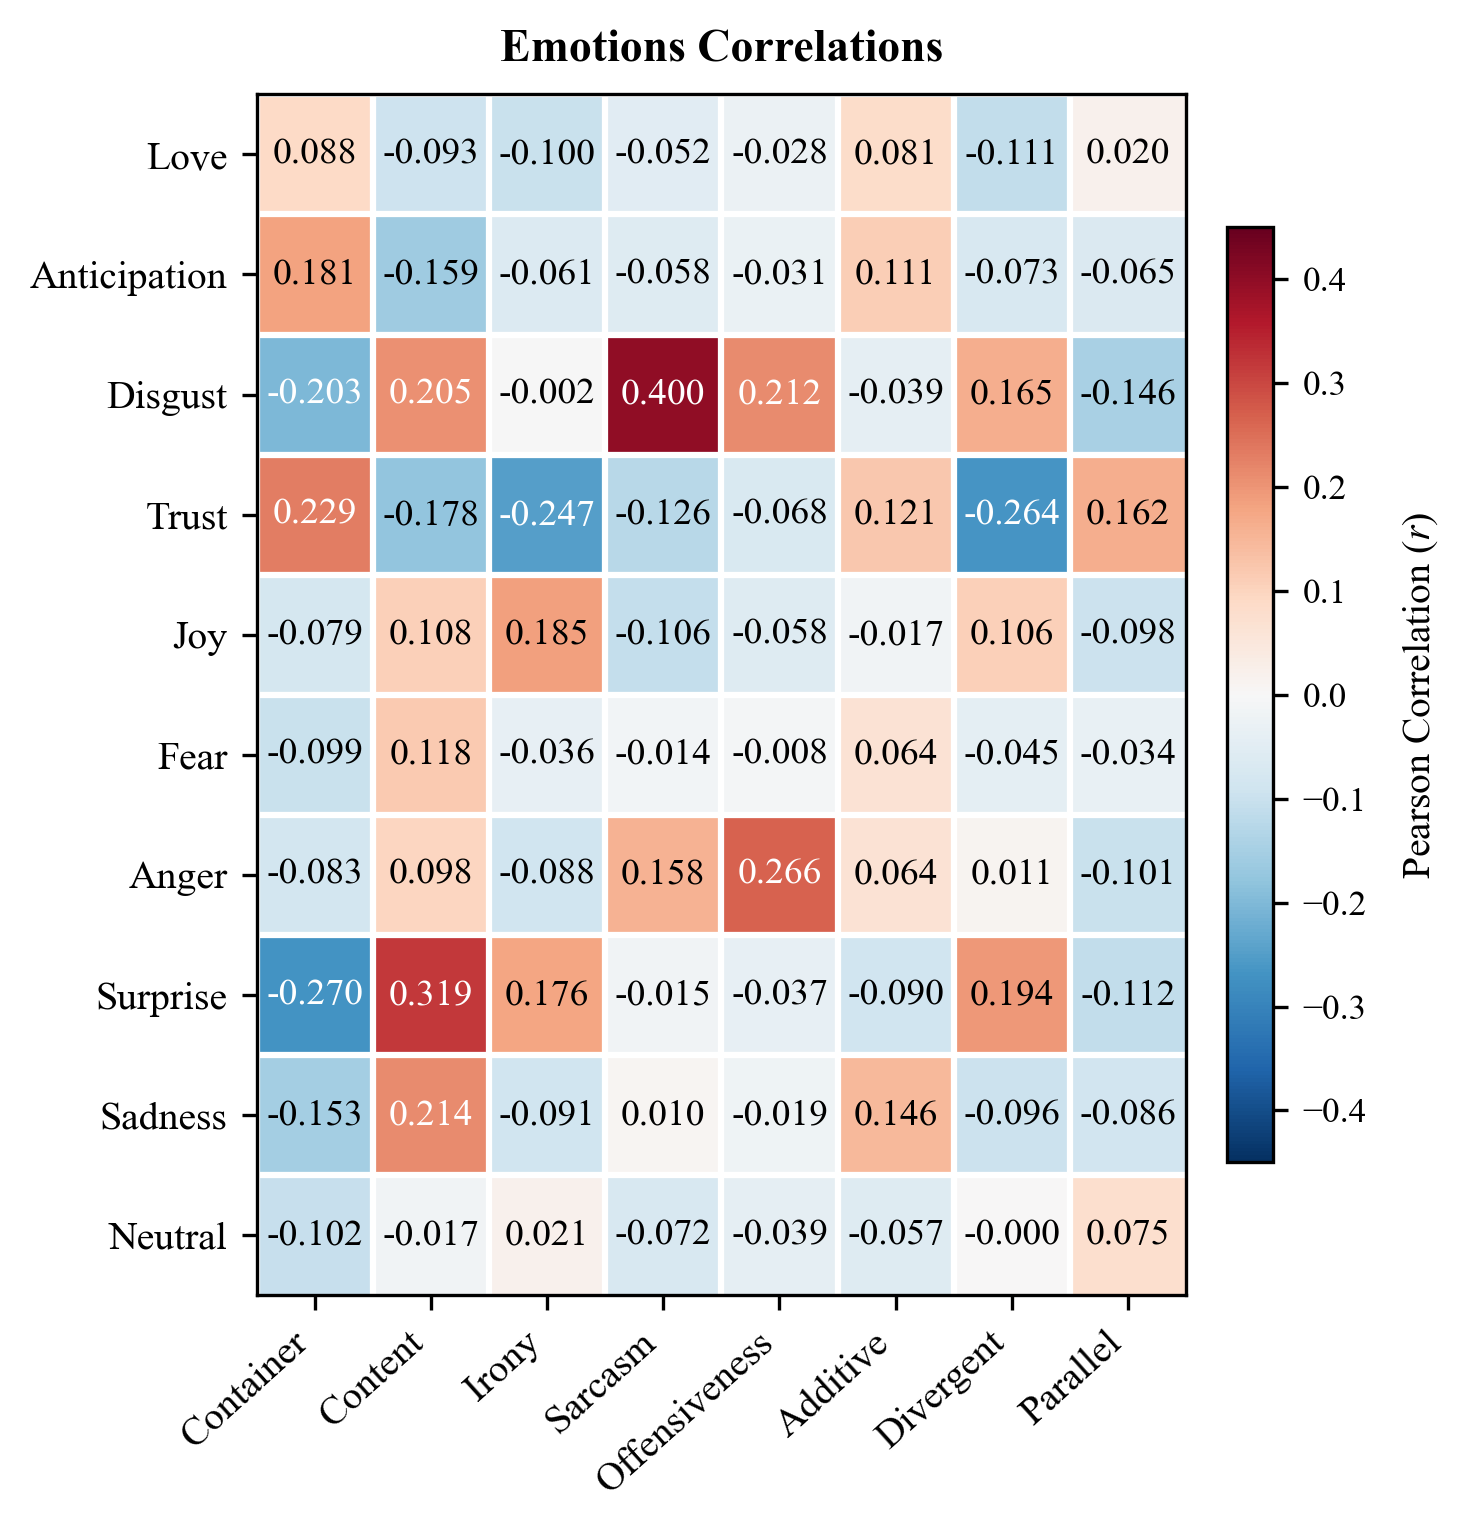
\includegraphics[width=0.92\columnwidth]{imgs/emotion_correlations_english.png}
\caption{Pearson correlation matrix between emotion labels and contextual dimensions (broadcast targets, figurative speech, and semiotic relations) in the Multimodal partition.}
\label{fig:emotions_correlations}
\end{figure}

\begin{figure*}[!t]
\centering
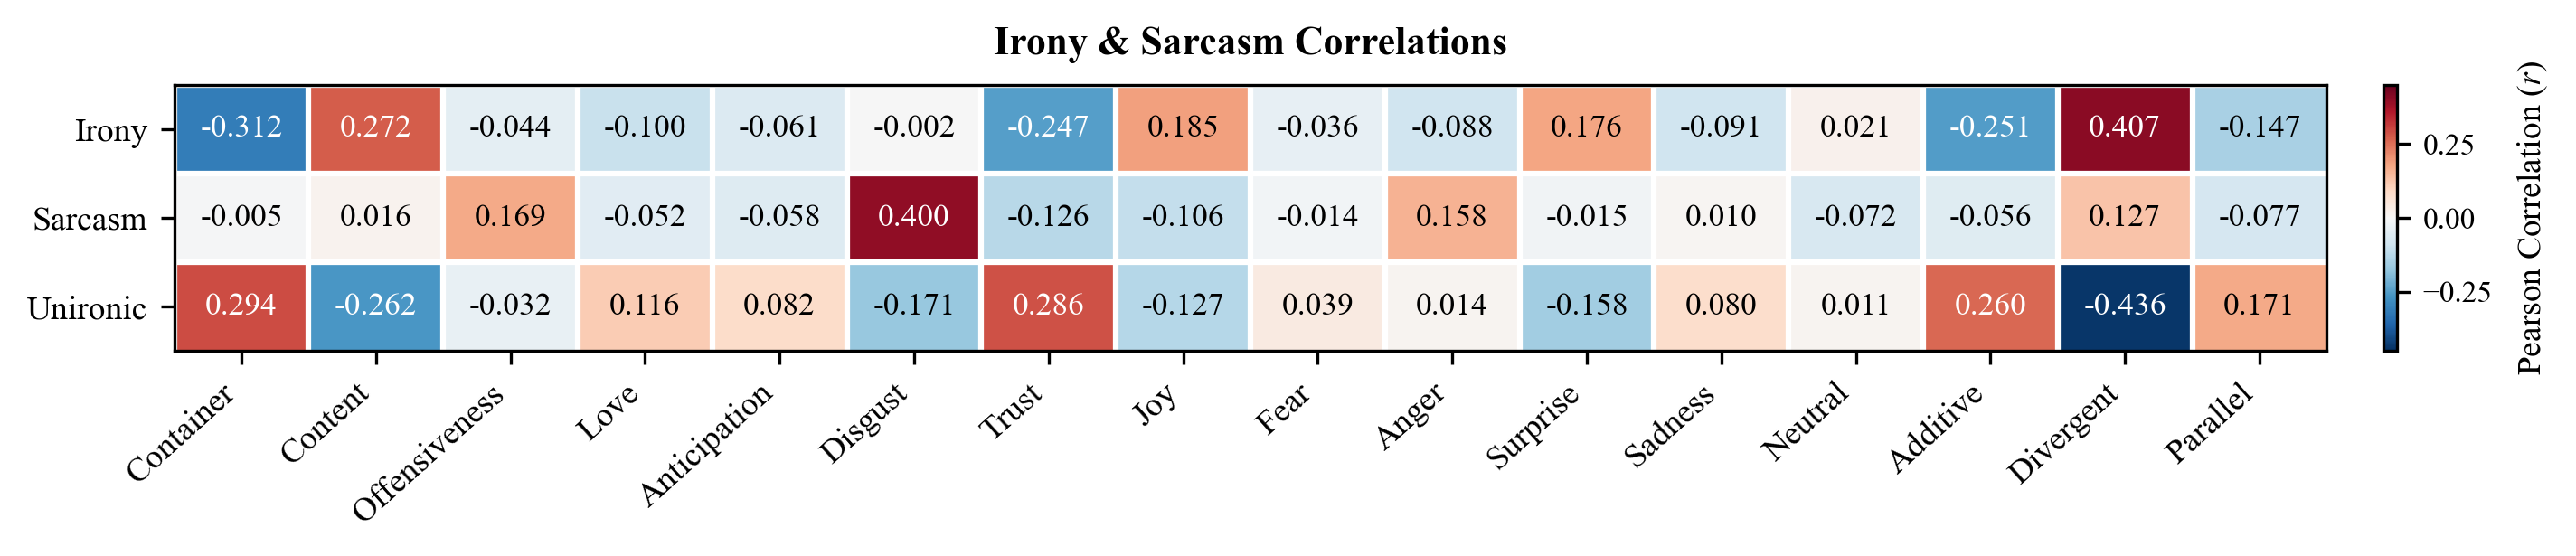
\includegraphics[width=\textwidth]{imgs/irony_correlations_english.png}
\caption{Pearson correlation matrix for the irony and sarcasm dimension across multi-level annotations within the Multimodal partition.}
\label{fig:irony_correlations}
\end{figure*}

\begin{figure*}[!t]
\centering
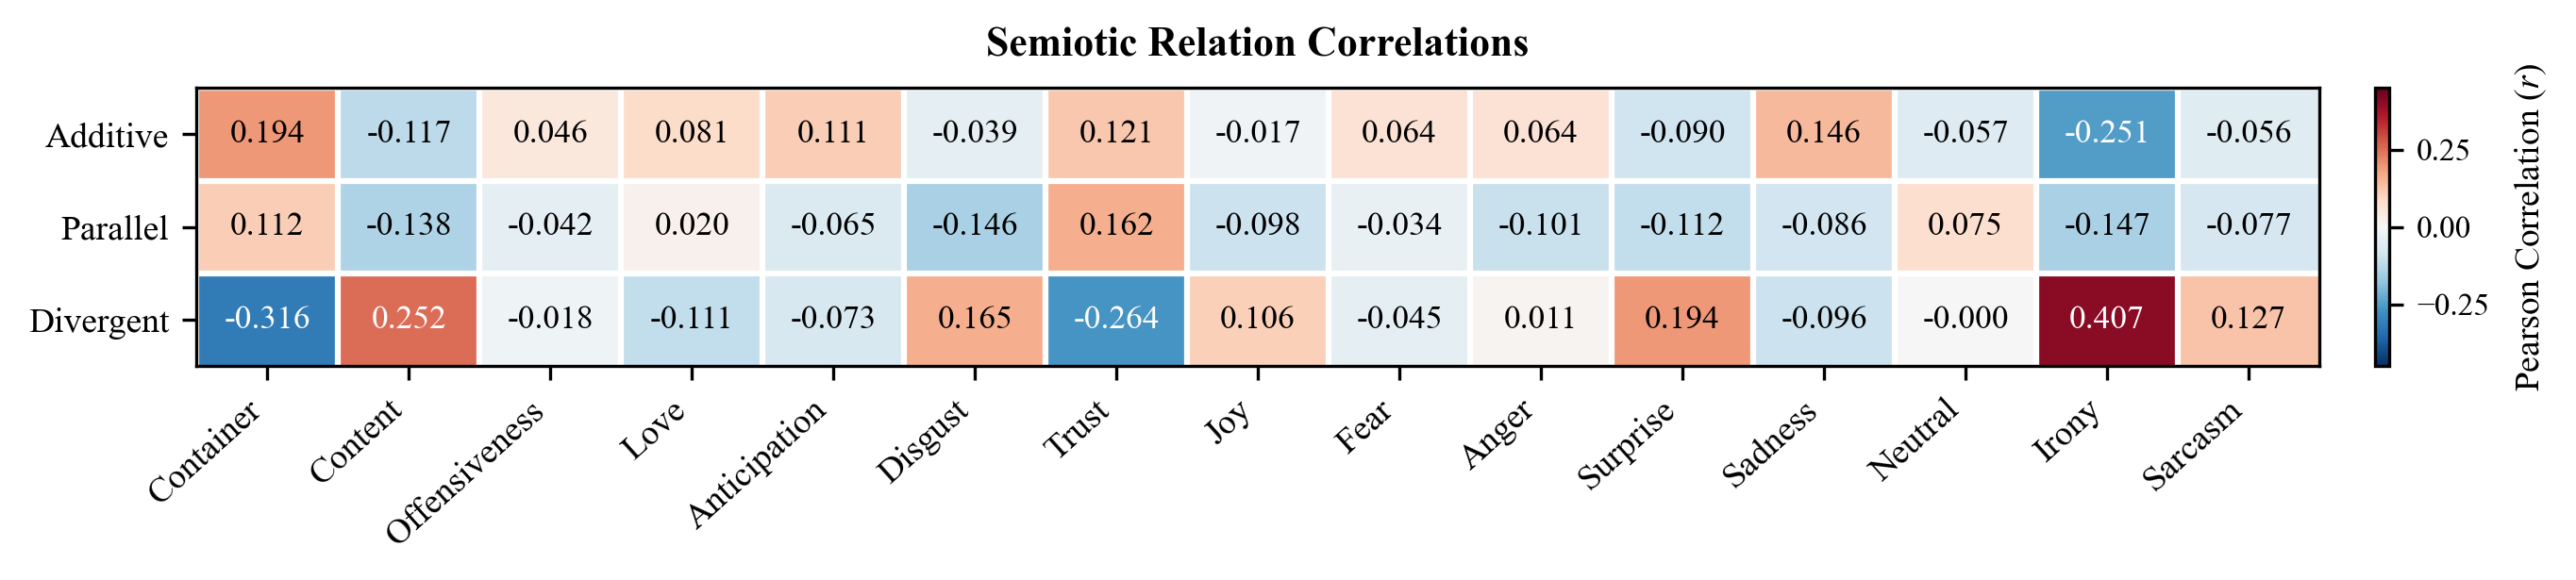
\includegraphics[width=\textwidth]{imgs/relation_correlations_english.png}
\caption{Pearson correlation matrix for semiotic text-image relations against contextual and affective markers in the Multimodal partition.}
\label{fig:relations_correlations}
\end{figure*}

Examining the correlation matrix for \textbf{Emotions} (Fig.~\ref{fig:emotions_correlations}), a clear dichotomy emerges between the \textit{Container} and \textit{Content} targets. Program-directed affective states (\textit{Trust} $r = 0.229$, \textit{Anticipation} $r = 0.181$) correlate positively with Container, indicating audience loyalty toward the show. Conversely, content-reactive emotions (\textit{Surprise} $r = 0.319$, \textit{Sadness} $r = 0.214$, \textit{Disgust} $r = 0.205$) associate with Content. Sarcasm also reveals a hostile pragmatic pattern, correlating positively with \textit{Disgust} ($r = 0.400$), offensive language ($r = 0.169$), and \textit{Anger} ($r = 0.158$).

Analyzing \textbf{Irony} (Fig.~\ref{fig:irony_correlations}), we observe that figurative speech relies fundamentally on semiotic contrast. Irony correlates with \textit{Divergent} text-image relations ($r = 0.407$), the \textit{Content} target ($r = 0.272$), and \textit{Joy} ($r = 0.185$), demonstrating that multimodal irony frequently arises from playful tension between the visual image and the written caption. Sincere posts (\textit{Unironic}), by contrast, correlate with \textit{Container} ($r = 0.294$), \textit{Trust} ($r = 0.286$), and complementary visual relations (\textit{Additive} $r = 0.260$, \textit{Parallel} $r = 0.171$).

Semiotic relations (Fig.~\ref{fig:relations_correlations}) confirm that divergent pairings drive social media irony: Divergent posts correlate positively with \textit{Irony} ($r = 0.407$), \textit{Content} ($r = 0.252$), and \textit{Surprise} ($r = 0.194$). In contrast, the \textit{Additive} relation associates with \textit{Container} ($r = 0.194$) and narrative elaboration, while the \textit{Parallel} relation exhibits minimal correlation with complex emotional states, reflecting literal and redundant text-image usage.
\section{Experimental Design}
\label{sec:experimental_design}

\begin{figure*}[!t]
\centering
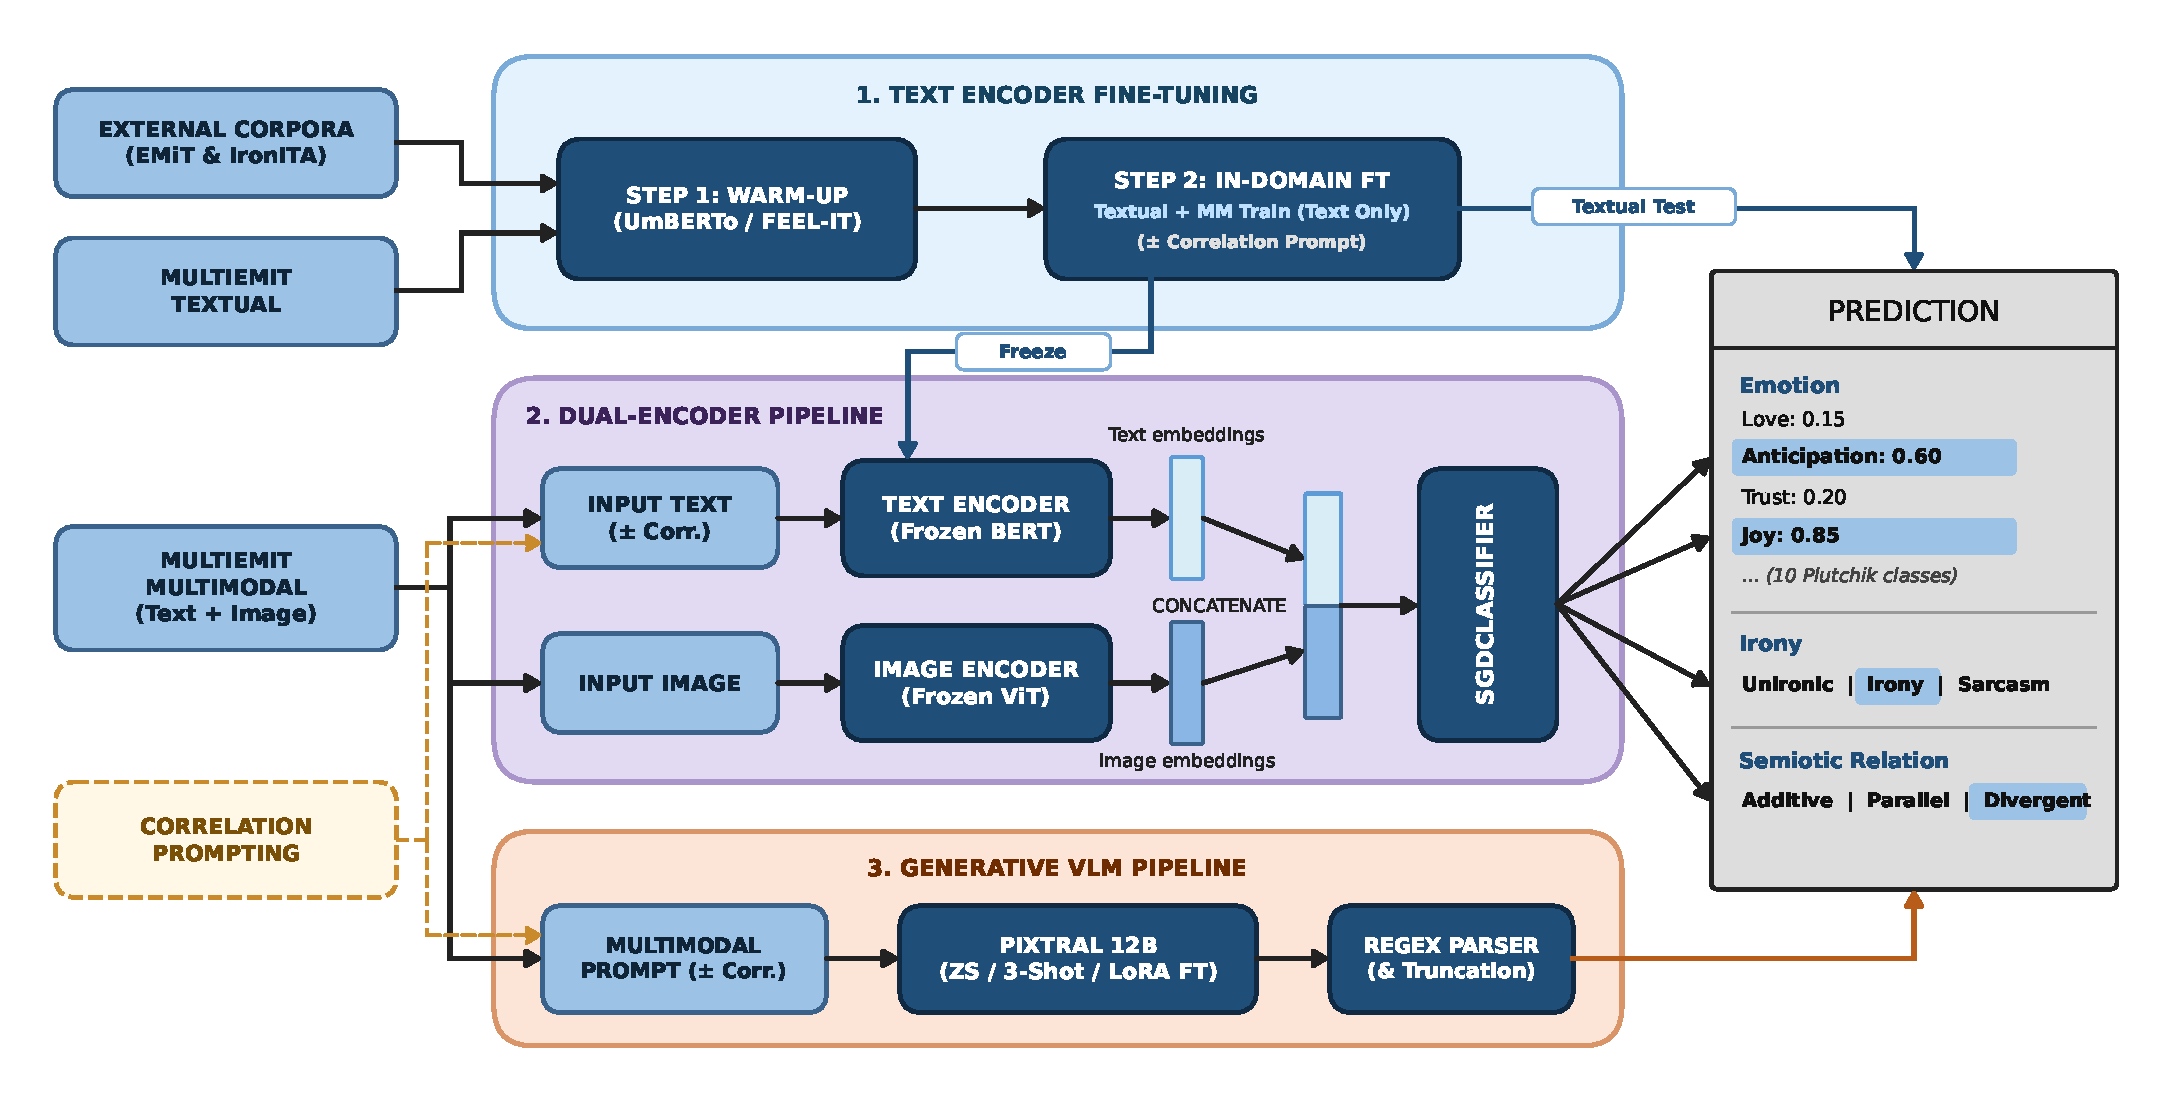
\includegraphics[width=0.92\textwidth]{imgs/pipeline_architecture.pdf}
\caption{Schematic overview of the MultiEMiT experimental pipeline. Text encoders are fine-tuned sequentially in two steps (warm-up on external corpora followed by in-domain fine-tuning on combined MultiEMiT text). For multimodal classification, frozen representations from the fine-tuned text encoder and a frozen ViT image encoder are concatenated into a joint vector ($d=1536$) and classified with linear SVMs (\texttt{SGDClassifier}). The generative pipeline benchmarks Pixtral 12B under zero-shot, few-shot, and LoRA fine-tuning. Correlation prompting optionally verbalizes gold auxiliary annotations across both paradigms.}
\label{fig:pipeline_architecture}
\end{figure*}

This section details the methodology used to probe the MultiEMiT corpus on three tasks: Emotion Detection (multi-label over ten categories), Irony Detection (three mutually exclusive classes: \textit{Unironic}, \textit{Irony}, \textit{Sarcasm}), and Semiotic Relation Detection (\textit{Additive}, \textit{Parallel}, \textit{Divergent}). Rather than maximizing performance, the experiments are designed to measure how much information each modality and each annotation layer carries. All MultiEMiT partitions were split with a fixed 80/20 ratio (\texttt{random\_state=42}): the textual dataset into 1,618 training and 405 test posts, and the multimodal dataset into 516 training and 129 test posts. The same multimodal test split is used for all discriminative and generative models. Given the size of the corpus, no separate validation split was held out. External corpora were used for training only, and all results are computed exclusively on MultiEMiT test instances. An overview of the complete experimental workflow across text-only fine-tuning, discriminative dual-encoding, and generative vision--language modeling is illustrated in Fig.~\ref{fig:pipeline_architecture}.

Because of severe class imbalance, raw accuracy is a misleading indicator of model quality. \textbf{Macro $F_1$} is our primary metric, as it weights all classes equally and penalizes poor performance on minority labels; \textbf{Micro $F_1$} is reported alongside it in the discriminative baseline tables. For reference against class skew, a trivial majority-class baseline on the multimodal test set predicting \textit{Unironic} for all instances achieves an artificially inflated Micro $F_1$ of $0.806$ but a Macro $F_1$ of only $0.298$; on relation detection, predicting the dominant \textit{Additive} class yields Micro $F_1 = 0.527$ and Macro $F_1 = 0.230$. For breakdowns across semiotic subsets (Section~\ref{sec:results}), we report Micro $F_1$ to maintain statistical stability on small subsets; for the single-label irony task, subset Micro $F_1$ equals accuracy, while for relation detection, where subsets coincide with target classes, we report per-class $F_1$. Discriminative results are averaged over three training seeds (42, 123, 456), which control encoder fine-tuning, data ordering, and the linear classifier, while the data splits are kept fixed; this isolates training variability from test-set sampling.

For Emotion and Irony Detection, text encoders were trained in two sequential steps (Fig.~\ref{fig:pipeline_architecture}, top). In \textit{Step~1} (domain warm-up), the encoder was fine-tuned on the union of the MultiEMiT textual training split (1,618 posts) and the full external corpus: EVALITA 2023 EMiT \cite{emit} (5,966 posts) for emotion, and IronITA \cite{ironita2018} (4,849 posts) for irony. In \textit{Step~2}, the Step~1 checkpoint was further fine-tuned on the textual and multimodal training splits (2,134 posts, text only), either on raw text or with correlation-prompted inputs (described below). For Semiotic Relation Detection, where annotations exist only for posts with paired media, UmBERTo encoders were fine-tuned on the multimodal training split, with and without correlation prompts.

Emotion encoders start from the FEEL-IT emotion classifier \cite{bianchi2021feel} (\texttt{MilaNLProc/feel-it-italian-emotion}, based on UmBERTo), while irony and relation encoders start from UmBERTo \cite{musixmatch-2020-umberto}, a RoBERTa-based model \cite{liu2019roberta} pre-trained on Italian Common Crawl with whole-word masking. All encoders were fine-tuned for 10 epochs (batch size 16, learning rate $2\times10^{-5}$, weight decay 0.01, maximum length 128 tokens). For textual emotion inference, labels with sigmoid probability $\geq 0.40$ are predicted; if none exceeds the threshold, the top-ranked label is selected, together with the second one when their probability gap is $\leq 0.10$. The classification heads of these fine-tuned encoders provide the text-only results on the textual test set.

To capture cross-modal interactions, we implemented a discriminative Dual-Encoder pipeline (Fig.~\ref{fig:pipeline_architecture}, middle) operating on frozen features. The last-layer \texttt{[CLS]} embedding of the fine-tuned text encoder (768-d) \cite{devlin2019bert} and the last-layer \texttt{[CLS]} embedding of ViT-Base-224 (\texttt{google/vit-base-patch16-224}) \cite{dosovitskiy2021vit} (768-d; images standardized to $224\times224$ pixels via bilinear resizing without aspect-ratio padding and ImageNet-normalized \cite{deng2009imagenet}) are concatenated, without rescaling, into a 1,536-dimensional vector. A linear SVM (\texttt{SGDClassifier} \cite{pedregosa2011scikit}, squared hinge loss, L2 penalty, balanced class weights) is fitted on the multimodal training split, wrapped in a \texttt{ClassifierChain} \cite{read2011classifier} for multi-label emotion detection to model label interdependencies, and applied directly to the single-label irony and relation tasks. The \textit{text only} configurations apply the same classifier to the text embedding alone, isolating the contribution of the visual features.

Motivated by the cross-layer dependencies observed in Section~\ref{sec:dataset_analysis}, we developed a \textit{Correlation Prompting} strategy tailored to each model family. For discriminative encoders, the gold annotations of the non-target layers are verbalized and prepended to the post (e.g., \textit{``ma soleil è con sua nonna?''} is preceded by \textit{``il seguente testo contiene ironia [...]''}), so that supervised training can learn their statistical association with the target labels. For Emotion and Irony Detection, the verbalization covers the emotion, irony, offensiveness, and target layers (excluding the task being predicted) but not the semiotic relation, which is annotated only for posts with paired media. This keeps the input format identical across the textual and multimodal partitions and prevents image-derived information from entering the text-only configurations; the effect of additionally verbalizing the relation for multimodal posts is reported as an ablation. For Semiotic Relation Detection, all four remaining layers are verbalized. Because gold auxiliary labels are supplied at both training and inference time, correlation prompting is an \textit{oracle} setting that estimates the informativeness of each annotation layer rather than a deployable system.

To compare specialized discriminative systems with modern generative vision--language models, we benchmarked \textbf{Pixtral 12B} \cite{pixtral} (Fig.~\ref{fig:pipeline_architecture}, bottom), an open-weights multimodal language model based on Mistral Nemo with a dedicated 400M-parameter vision encoder. Pixtral was fine-tuned and evaluated exclusively on the multimodal partition, using the same test split as the Dual-Encoder. Since its training data and input format differ from those of the discriminative pipeline, this comparison contrasts modeling paradigms on a shared test set rather than constituting a controlled ablation. In correlation-prompted settings, each post is preceded by the verbalized annotations of the other layers, always including the semiotic relation for emotion and irony, at both training and inference time. A fine-tuned encoder can learn statistical associations between these annotations and the target labels, but a model used in zero- or few-shot inference cannot. We therefore emulate this learned knowledge by additionally stating in the task instruction the main Pearson correlations between the target labels and the other annotation layers (e.g., \textit{``Disgust correlates with Sarcasm. Anger correlates with Offensivity.''}; see Section~\ref{sec:dataset_analysis}). To measure prompt sensitivity, we designed five variants spanning three correlation intensity thresholds: \textbf{Short} ($|r| \ge 0.25$), \textbf{Medium} ($|r| \ge 0.20$), and three \textbf{Long} formulations (\textit{long\_v1}, \textit{long\_v2}, \textit{long\_v3}; $|r| \ge 0.15$). Following findings from the BRIGHTER benchmark \cite{brighter_project} showing that multilingual LLMs exhibit stronger instruction adherence when prompted in English, all generative instructions were formulated in English.

For all Pixtral experiments, input images were standardized to a fixed resolution of $336 \times 336$ pixels via the model's image processor (\texttt{size = \{"height": 336, "width": 336\}}). We evaluated Pixtral across three regimes: Zero-Shot Prompting across all five correlation variants and an unprompted baseline; Few-Shot (Three-Shot) Prompting \cite{brown2020language} for Semiotic Relation Detection, where three complete multimodal examples were included in the prompt as a design choice to help the model with a newer and more specialized task that it is less likely to have encountered during pre-training compared to emotions or irony; and LoRA Fine-Tuning on the MultiEMiT multimodal training set ($r=16$, $\alpha=32$, RSLoRA \cite{hu2021lora, kalajdzievski2023rank}, all linear target modules, dropout $0.1$), adapting 66,322,432 parameters out of 12.75 billion (0.52\% trainable) with per-device batch size 1, 8 gradient accumulation steps, learning rate $3 \times 10^{-5}$, FP16 mixed precision, and gradient checkpointing over 2 epochs. To account for generation variance, each Pixtral configuration was evaluated at two decoding temperatures ($T=0.1$ and $T=0.9$) with 3 independent runs per setting (reporting mean scores). To extract predictions from the generated text, we used regular expressions to match valid label names. After fine-tuning on emotion detection, Pixtral often continued generating long or repeated lists of emotions instead of stopping after one or two labels. Because regex matching extracted all mentioned labels, these extra guesses lowered performance. By comparing the raw outputs with the gold labels, we noticed that the emotions were usually listed from most likely to least likely, so we added a truncation parameter that keeps only the first $n=2$ distinct emotions, matching the maximum of two emotions requested in the prompt.
\section{Results and Discussion}
\label{sec:results}

This section evaluates unimodal and multimodal architectures on Emotion Detection, Irony Detection, and Semiotic Relation Detection. Rather than targeting state-of-the-art performance, we use these baselines to probe the corpus: we measure the contribution of visual features (text-only vs.\ Dual-Encoder), the informativeness of the auxiliary annotation layers (correlation prompting), and the behavior of Pixtral 12B, also disaggregated across semiotic subsets. Discriminative results are means over three training seeds; we describe an effect as consistent when it holds in all three seeds.

\subsection{Emotion Detection}
\label{sec:emotion_results}

Emotion detection represents the most challenging benchmark due to the high cardinality of the ten-class label space and the multi-label nature of affective expression in social media. Exploratory experiments attempting to collapse co-occurring emotions into single-label multiclass dyads under Plutchik's taxonomy or Ekman's basic emotions \cite{ekman1992argument} suffered from acute class sparsity and severe majority-class collapse. Recasting the task as a 10-dimensional multi-label binary problem over Plutchik's primary emotions (plus \textit{Love} and \textit{Neutral}) resolved this structural bottleneck.

Table~\ref{tab:emotion_baselines} summarizes the discriminative baselines. On the textual test set, the Step~1 encoder reaches a Macro $F_1$ of $0.506$. Further in-domain fine-tuning on raw text brings only a marginal change ($0.515$), whereas fine-tuning with correlation prompts raises performance to $0.530$, outperforming the raw Step~2 encoder in all three seeds.

On the multimodal test set, the text-only probe reaches $0.424$. Neither visual features ($0.432$) nor correlation prompts ($0.426$) improve it consistently on their own, but their combination yields $0.505$ ($+8.1$ points), exceeding both single-source configurations in every seed. Visual context and auxiliary annotations are therefore complementary for emotion: telling the classifier the target and figurative labels narrows down the ten emotions to a few likely candidates, allowing the visual features to separate categories with strong contextual ties such as \textit{Disgust} ($0.418 \rightarrow 0.589$) and \textit{Surprise} ($0.242 \rightarrow 0.379$). An inspection of the per-emotion confusion matrices confirms that this gain stems from genuine recovery of difficult affective instances rather than decision-threshold shifts: true positives increase from $7.0$ to $10.7$ for \textit{Disgust} (recall $37\% \rightarrow 56\%$) and from $3.7$ to $6.0$ for \textit{Surprise} (recall $23\% \rightarrow 38\%$), while false positive rates remain stable.

The ablation in Table~\ref{tab:emotion_baselines} shows the effect of also verbalizing the semiotic relation. On the textual test set, an encoder trained with the relation on its multimodal training rows improves to $0.544$, but on the multimodal test set the corresponding Dual-Encoder drops to $0.458$, below the configuration without the relation in all three seeds. Since the relation describes how text and image interact, it partly duplicates the information carried by the visual features rather than complementing it.

\begin{figure*}[!t]
\centering
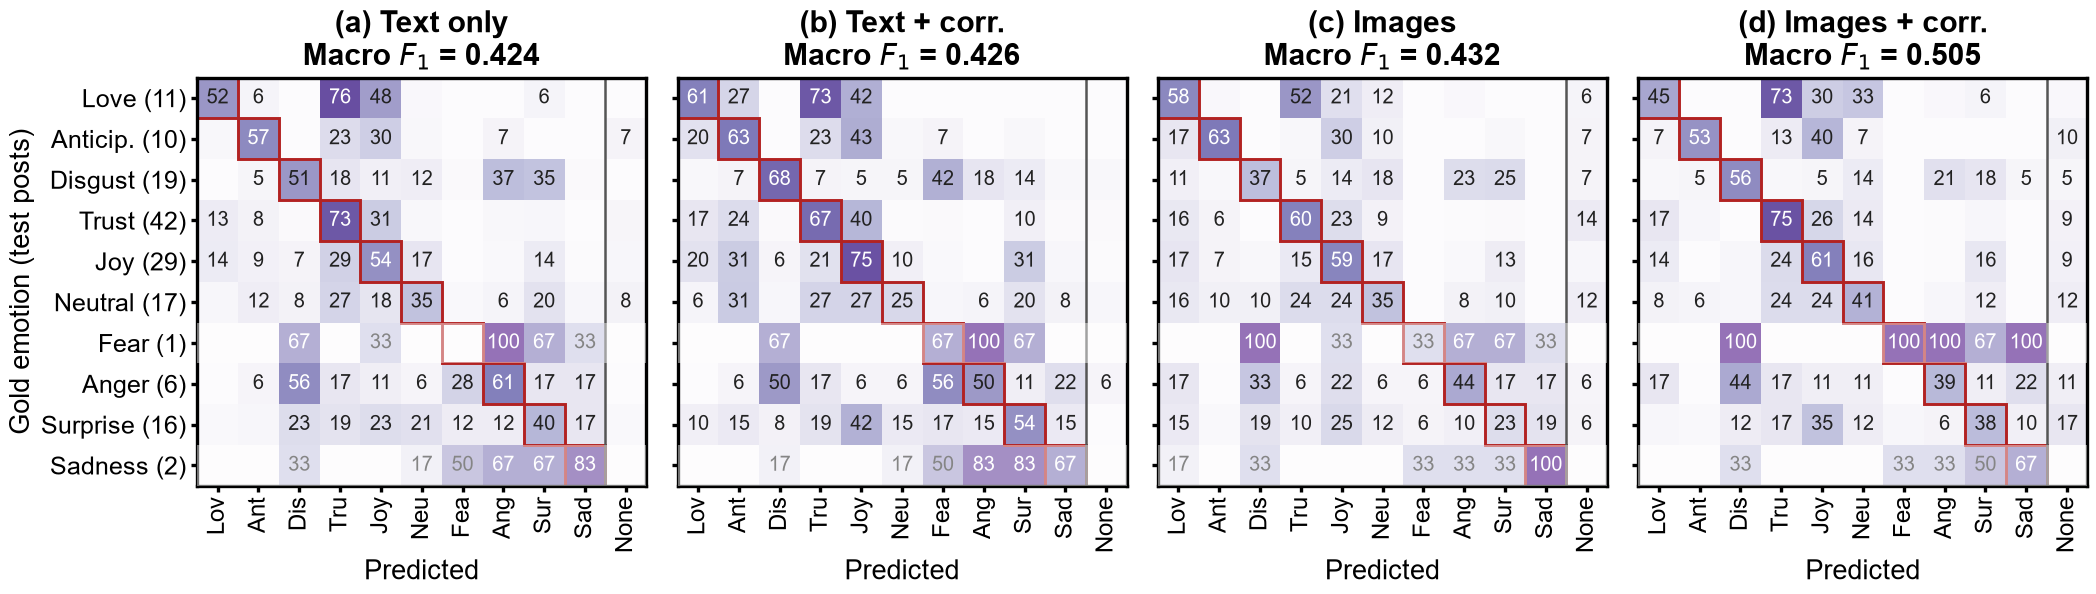
\includegraphics[width=\textwidth]{imgs/confusion_matrices_emotion.png}
\caption{Emotion detection on the multimodal test set ($N=129$), mean of three seeds. Each row is a gold emotion (number of test posts in brackets) and each cell is the percentage of those posts for which the column label was predicted; \textit{None} means that no label was predicted. Because a post can carry several emotions, rows can add up to more than 100\%. The red frame marks the correct label. \textit{Fear} and \textit{Sadness} have only 1 and 2 test posts and are shown faded.}
\label{fig:confusion_emotion}
\end{figure*}

Figure~\ref{fig:confusion_emotion} shows where these differences come from. Correlation prompts used on text alone add labels that the posts do not carry (Fig.~\ref{fig:confusion_emotion}b): the classifier predicts \textit{Fear} 14.3 times per run, against 3.3 without prompts and a single gold post, and 42\% of the \textit{Disgust} posts receive it. This raises the \textit{Disgust} recall from 51\% to 68\% but leaves the Macro $F_1$ unchanged. When images are added (Fig.~\ref{fig:confusion_emotion}d), \textit{Fear} falls back to 1.7 predictions and \textit{Disgust} is still recognized more often than without prompts (56\% against 37\% for the images alone), so the visual features appear to filter out part of what the prompt adds. Two groups of emotions remain confused in every setting: \textit{Love}, \textit{Trust}, and \textit{Joy} (\textit{Love} posts are labelled \textit{Trust} in 52\% to 76\% of the cases), and \textit{Disgust}, \textit{Anger}, and \textit{Surprise} (37\% and 35\% of \textit{Disgust} posts are labelled \textit{Anger} and \textit{Surprise} by the text-only model, 21\% and 18\% with images and prompts). Finally, the larger classes attract predictions: \textit{Trust} and \textit{Joy} are predicted 52.7 and 34.7 times by the text-only model, against 42 and 29 gold posts.

\begin{table}[!t]
\centering
\caption{Discriminative Baseline Performance in Emotion Detection (Mean of Three Seeds)}
\label{tab:emotion_baselines}
\footnotesize
\renewcommand{\arraystretch}{1.05}
\begin{tabular}{l c c}
\hline
\textbf{Configuration} & \textbf{Macro $F_1$} & \textbf{Micro $F_1$} \\
\hline
\multicolumn{3}{l}{\textit{Textual Test Set}} \\
Step 1 (EMiT + MultiEMiT) & 0.506 & 0.529 \\
Step 2 without correlations & 0.515 & 0.528 \\
Step 2 with correlations & \textbf{0.530} & \textbf{0.555} \\
\hline
\multicolumn{3}{l}{\textit{Multimodal Test Set}} \\
Text only & 0.424 & 0.492 \\
Text only with correlations & 0.426 & 0.499 \\
With images & 0.432 & 0.475 \\
With images and correlations & \textbf{0.505} & \textbf{0.529} \\
\hline
\multicolumn{3}{l}{\textit{Ablation: Relation Added to the Prompt}} \\
Step 2 with correlations (textual)$^{*}$ & 0.544 & 0.557 \\
Text only with correlations + relation & 0.439 & 0.515 \\
With images, correlations + relation & 0.458 & 0.520 \\
\hline
\multicolumn{3}{p{0.92\columnwidth}}{\footnotesize $^{*}$Relation verbalized on multimodal training rows only; textual test posts have no relation annotation.} \\
\end{tabular}
\end{table}

Turning to generative models (Table~\ref{tab:emotion_pixtral}), we selected the \textit{short} and \textit{long\_v1} templates for LoRA fine-tuning, as \textit{long\_v1} achieved the highest mean Macro $F_1$ across both decoding temperatures among the long zero-shot prompts. Fine-tuned Pixtral 12B (\textit{long\_v1}, $n=2$, $0.426$ at $T=0.1$) performs on par with the Dual-Encoder without correlations ($0.432$), but remains clearly below the correlation-prompted Dual-Encoder ($0.505$). The gap persists when the Dual-Encoder receives the same annotation layers as Pixtral, including the relation ($0.458$).

\begin{table}[!t]
\centering
\caption{Pixtral 12B versus Dual-Encoder in Emotion Detection ($T=0.1$ and $T=0.9$)}
\label{tab:emotion_pixtral}
\footnotesize
\renewcommand{\arraystretch}{0.92}
\begin{tabular}{l l c c}
\hline
\textbf{Model} & \textbf{Configuration} & \textbf{$T = 0.1$ $F_1$} & \textbf{$T = 0.9$ $F_1$} \\
\hline
\multicolumn{4}{l}{\textit{Discriminative Multimodal (Dual-Encoder)}} \\
BERT-ViT & FT (No Corr.) & 0.432 & 0.432 \\
BERT-ViT & FT (Corr.) & \textbf{0.505} & \textbf{0.505} \\
BERT-ViT & FT (Corr. + Rel.)$^{\dagger}$ & 0.458 & 0.458 \\
\hline
\multicolumn{4}{l}{\textit{Generative (Pixtral 12B)}} \\
Pixtral (long\_v1) & FT ($n=2$) & \textbf{0.426} & 0.359 \\
Pixtral (short) & FT ($n=2$) & 0.397 & \textbf{0.373} \\
Pixtral (short) & FT (all predictions) & 0.318 & 0.312 \\
Pixtral (short) & ZS (With Corr.) & 0.291 & 0.251 \\
Pixtral (long\_v1) & ZS (With Corr.) & 0.275 & 0.266 \\
Pixtral (medium) & ZS (With Corr.) & 0.269 & 0.262 \\
Pixtral (long\_v2) & ZS (No Corr.) & 0.266 & 0.237 \\
Pixtral (long\_v1) & ZS (No Corr.) & 0.261 & 0.261 \\
Pixtral (short) & ZS (No Corr.) & 0.261 & 0.291 \\
Pixtral (long\_v3) & ZS (With Corr.) & 0.258 & 0.262 \\
Pixtral (medium) & ZS (No Corr.) & 0.254 & 0.250 \\
Pixtral (long\_v2) & ZS (With Corr.) & 0.253 & 0.286 \\
Pixtral (long\_v1) & FT (all predictions) & 0.238 & 0.290 \\
Pixtral (long\_v3) & ZS (No Corr.) & 0.220 & 0.215 \\
\hline
\multicolumn{4}{p{0.95\columnwidth}}{\footnotesize Macro $F_1$. Dual-Encoder values are means over three training seeds and do not depend on decoding temperature; Pixtral values are means over three generation runs. Correlation-prompted Pixtral receives the per-instance annotations of the other layers (including the semiotic relation) and corpus-level correlation rules in the instruction. $^{\dagger}$Dual-Encoder input matched to Pixtral (relation included).} \\
\end{tabular}
\end{table}

\begin{table}[!t]
\centering
\caption{Impact of Truncation Parameter ($n$) on Pixtral Emotion Detection Performance}
\label{table:truncation_parameter}
\footnotesize
\begin{tabular}{c c}
\hline
\textbf{Number of Predictions ($n$)} & \textbf{Mean Macro $F_1$} \\
\hline
1 & 0.338 \\
2 & \textbf{0.389} \\
3 & 0.339 \\
4 & 0.325 \\
5 & 0.308 \\
\hline
\end{tabular}
\end{table}

After fine-tuning on emotion detection, Pixtral often failed to stop generating and instead returned long or repetitive lists of emotions (for example, listing four or five emotions in a row, or repeating the same pair of emotions). Because we used regular expressions to match all valid emotion names in the output, these extra guesses produced many false positives and caused a clear drop in performance (shown in the \textit{all predictions} rows of Table~\ref{tab:emotion_pixtral}). When comparing these raw outputs against the gold standard, we noticed that the model generally listed the most likely emotions first. We therefore tested truncating the extracted list to the first $n$ distinct emotions ($n = 1, \dots, 5$). As shown in Table~\ref{table:truncation_parameter} (averaged across the fine-tuned \textit{short} and \textit{long\_v1} prompts over both temperatures), performance peaks at $n=2$ (Mean Macro $F_1 = 0.389$), which also matches the maximum of two emotions requested in the prompt and the typical number of emotions per post in the dataset.

Disaggregating performance across semiotic subsets (Table~\ref{tab:semiotic_subsets_all}) reveals a divergence between discriminative and generative paradigms.

\begin{table}[!t]
\centering
\caption{Performance across Semiotic Subsets (Additive, Parallel, Divergent) for All Three Tasks}
\label{tab:semiotic_subsets_all}
\footnotesize
\renewcommand{\arraystretch}{1.02}
\begin{tabular}{l c c c}
\hline
\textbf{Task \& Model Setting} & \textbf{ADD} & \textbf{PAR} & \textbf{DIV} \\
\hline
\multicolumn{4}{l}{\textit{Emotion Detection (Micro $F_1$-score)}} \\
Dual-Encoder (No corr.) & 0.56 & 0.52 & 0.30 \\
Dual-Encoder (With corr.) & \textbf{0.58} & \textbf{0.55} & 0.42 \\
Dual-Encoder (Corr. + relation)$^{\dagger}$ & 0.55 & 0.51 & \textbf{0.47} \\
Pixtral 12B Zero-Shot (No corr.) & 0.29 & 0.23 & 0.44 \\
Pixtral 12B Zero-Shot (With corr.) & 0.32 & 0.30 & 0.43 \\
Pixtral 12B Fine-tuned ($n=2$, No corr.) & 0.33 & 0.41 & 0.41 \\
\hline
\multicolumn{4}{l}{\textit{Irony Detection (Micro $F_1$-score / Accuracy)}} \\
Dual-Encoder (No corr.) & \textbf{0.88} & 0.90 & \textbf{0.63} \\
Dual-Encoder (With corr.) & 0.84 & 0.90 & 0.53 \\
Dual-Encoder (Corr. + relation)$^{\dagger}$ & \textbf{0.88} & 0.93 & 0.54 \\
Pixtral 12B Zero-Shot (No corr.) & 0.14 & 0.00 & 0.18 \\
Pixtral 12B Zero-Shot (With corr.) & 0.57 & 0.78 & 0.57 \\
Pixtral 12B Fine-tuned (No corr.) & 0.87 & \textbf{1.00} & 0.58 \\
\hline
\multicolumn{4}{l}{\textit{Semiotic Relation Detection (Per-Class $F_1$-score, Pixtral long\_v1)}} \\
Text-only Probe (No corr.) & 0.69 & 0.46 & 0.56 \\
Dual-Encoder (No corr.) & 0.67 & 0.43 & 0.56 \\
Text-only Probe (With corr.) & 0.68 & \textbf{0.57} & 0.56 \\
Dual-Encoder (With corr.) & \textbf{0.71} & 0.48 & 0.56 \\
Pixtral 12B Zero-Shot (No corr.) & 0.62 & 0.00 & 0.56 \\
Pixtral 12B Zero-Shot (With corr.) & 0.61 & 0.00 & 0.56 \\
Pixtral 12B Three-Shot (With corr.) & 0.60 & 0.17 & \textbf{0.64} \\
Pixtral 12B Fine-tuned (No corr.) & \textbf{0.71} & 0.28 & 0.60 \\
\hline
\multicolumn{4}{p{0.88\columnwidth}}{\footnotesize $^{\dagger}$Ablation; input matched to Pixtral.} \\
\end{tabular}
\end{table}

The \textbf{Dual-Encoder} performs best on the \textit{Additive} and \textit{Parallel} subsets and worst on the \textit{Divergent} one ($0.30$ without correlations). Redundant or complementary text--image content reinforces the concatenated signal, whereas the tension between modalities in Divergent posts is hard to resolve for a linear classifier over frozen features. Correlation prompting brings its largest gain precisely on Divergent posts ($0.30 \rightarrow 0.42$), where auxiliary annotations such as irony help disambiguate the intended affect; this is also the only subset where adding the relation helps further ($0.47$).

\textbf{Zero-shot Pixtral 12B} shows the inverse pattern, performing best on \textit{Divergent} ($0.44$) and worst on \textit{Parallel} posts ($0.23$). Divergent commentary mostly consists of reaction memes and satire dominated by salient states (\textit{Joy}, \textit{Surprise}, \textit{Disgust}), which internet-scale pre-training may allow Pixtral to decode without task-specific training: it surpasses the unprompted Dual-Encoder on this subset ($0.44$ vs.\ $0.30$) and the correlation-prompted one ($0.42$). On literal Parallel posts, zero-shot Pixtral lacks domain priors and recovers only after fine-tuning ($0.41$).

\subsection{Irony Detection}
\label{sec:irony_results}

Irony relies on pragmatic incongruity, which may arise within the text itself or between text and image \cite{schifanella2016multimodal, cai2019multimodal}. Irony encoders are initialized from UmBERTo and trained with the same two-step procedure, using IronITA \cite{ironita2018} in the warm-up step and evaluating exclusively on held-out MultiEMiT instances (Table~\ref{tab:irony_baselines}).

On the textual test set, in-domain fine-tuning is the main driver: Step~2 raises Macro $F_1$ from $0.449$ to $0.506$ in all three seeds. Correlation prompts bring a further gain to $0.533$, improving the \textit{Sarcasm} class ($F_1$ from $0.27$ to $0.31$, with only 8 sarcastic test posts) and making training markedly more stable across seeds.

\begin{figure*}[!t]
\centering
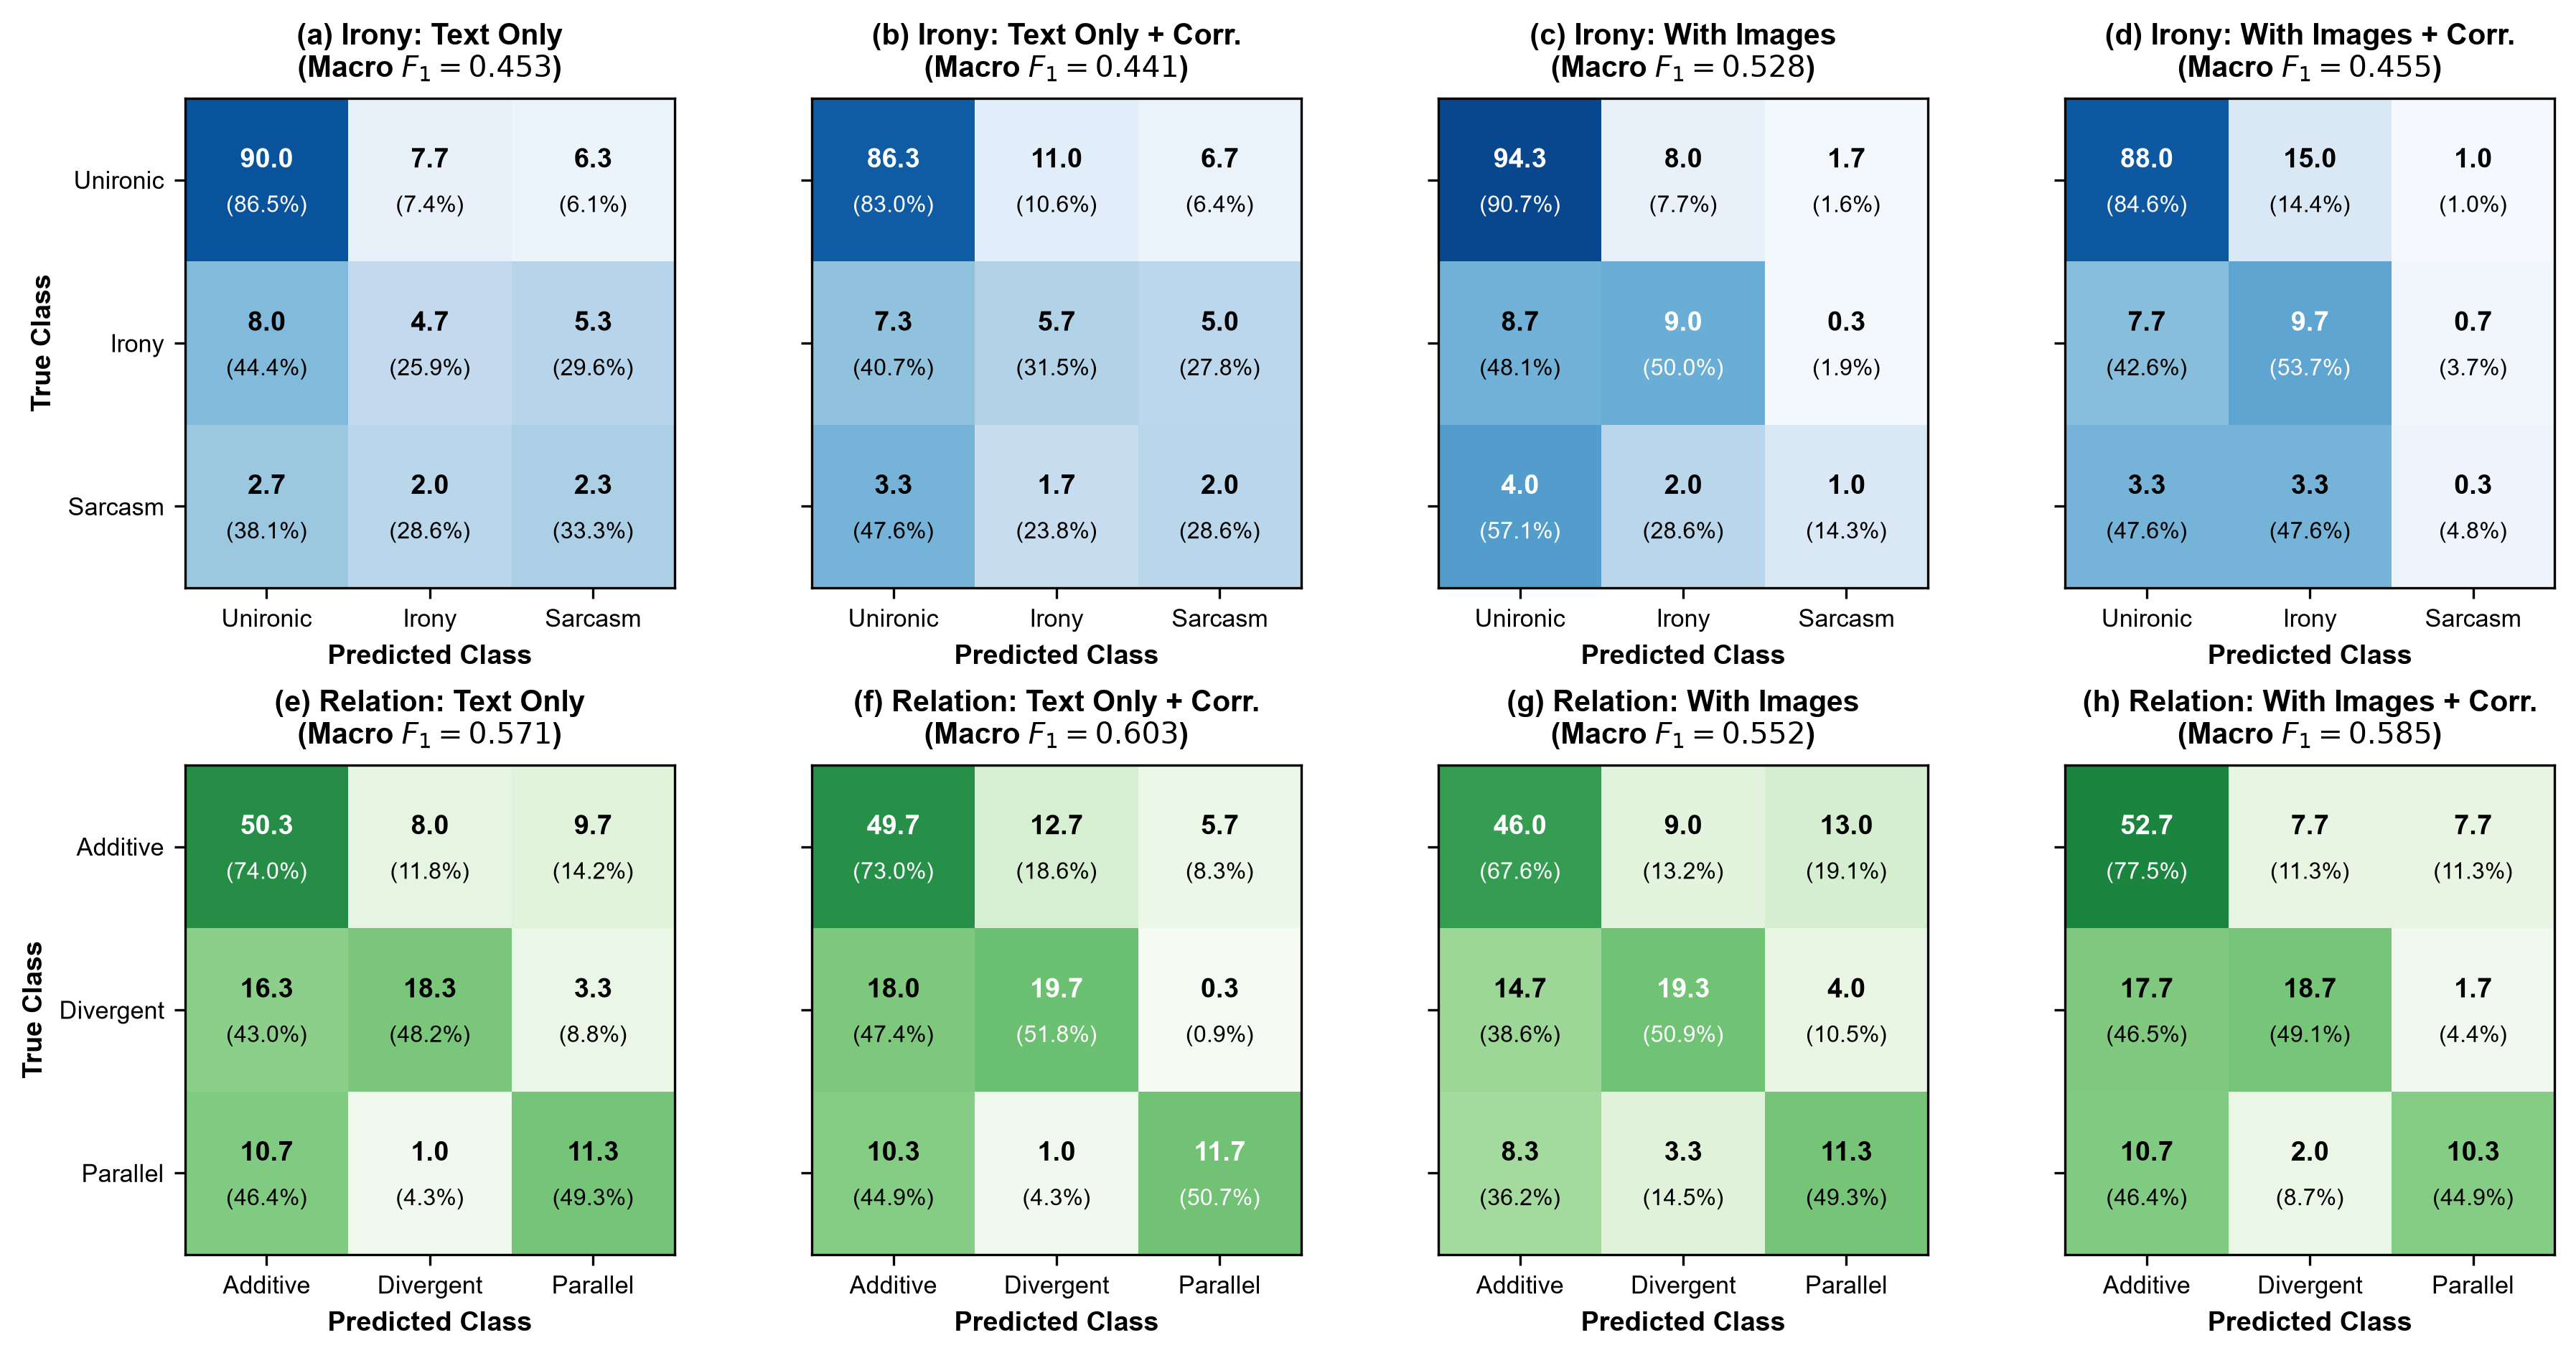
\includegraphics[width=0.98\textwidth]{imgs/confusion_matrices_irony_relation.png}
\caption{Three-seed averaged confusion matrices on the multimodal test set ($N=129$) for Irony Detection (top row, panels a--d) and Semiotic Relation Detection (bottom row, panels e--h), covering the complete $2\times2$ factorial design across input modalities (text only vs.\ with images) and correlation prompting. Each cell reports the mean number of test instances alongside the row-normalized percentage (true class recall). Cell shading reflects recall intensity.}
\label{fig:confusion_matrices}
\end{figure*}

On the multimodal test set, visual features provide the most robust effect observed in our study: the Dual-Encoder improves over the text-only probe from $0.453$ to $0.528$ ($+7.5$ points) in every seed, mainly by recognizing ironic posts (\textit{Irony} $F_1$ from $0.27$ to $0.49$). (For reference against severe class imbalance, a trivial majority-class baseline predicting \textit{Unironic} for all instances achieves an accuracy of $0.806$ but a Macro $F_1$ of only $0.298$, since minority figurative classes receive zero). This is consistent with the strong association between irony and Divergent text--image relations ($r = 0.407$, Section~\ref{sec:dataset_analysis}): part of the incongruity that defines multimodal irony is only observable in the image. Correlation prompts, by contrast, do not help on multimodal posts ($0.441$ text only, $0.455$ with images), and largely cancel the visual gain. Although the textual and multimodal correlation matrices share the same positive and negative signs, the target distribution shifts between partitions: in the textual dataset (which makes up 75.8\% of Step~2 training), \textit{Container} is a minority class (38.7\%) and 83.7\% of \textit{Container} posts are \textit{Unironic}, whereas in the multimodal dataset \textit{Container} becomes the majority (61.2\%) because viewers attach broadcast screenshots, and 27.8\% of ironic test posts (and 57.1\% of sarcastic test posts) target the \textit{Container}. When the prompt explicitly states that a post targets the \textit{Container}, the text encoder relies on the textual prior and pushes predictions toward \textit{Unironic}, overriding the visual contrast. Adding the relation to the prompt lowers performance further ($0.432$) and suppresses \textit{Sarcasm} entirely ($F_1 = 0$ in every seed): in the multimodal training split, \textit{Divergent} posts co-occur with \textit{Irony} 55 times versus \textit{Sarcasm} only 7 times, causing the linear classifier to favor \textit{Irony} whenever the relation is provided. With 25 ironic or sarcastic posts in the multimodal test set, these differences should be interpreted with caution.

An inspection of the confusion matrices (Fig.~\ref{fig:confusion_matrices}, top row) clarifies the exact error dynamics driving these shifts across the four factorial conditions. In the text-only probe (Fig.~\ref{fig:confusion_matrices}a), true ironic posts are correctly detected only 25.9\% of the time (4.7 out of 18 posts) and are frequently confused with sarcasm (29.6\%, 5.3 posts). Adding correlation prompts to text alone (Fig.~\ref{fig:confusion_matrices}b) yields only modest recall gains for irony (31.5\%, 5.7 posts) while increasing false alarms on sincere posts (from 7.4\% to 10.6\%, 11.0 posts). Incorporating visual representations in the Dual-Encoder without prompts (Fig.~\ref{fig:confusion_matrices}c) produces the sharpest behavioral improvement: true irony recall doubles to 50.0\% (9.0 posts) and confusion with sarcasm is virtually eliminated (dropping from 29.6\% to 1.9\%, 0.3 posts), while false sarcastic alarms on sincere instances drop to 1.6\%. When correlation prompts are combined with images (Fig.~\ref{fig:confusion_matrices}d), the model over-triggers irony on sincere posts: unironic false alarms jump to 14.4\% (15.0 posts), explaining the drop in precision and overall Macro $F_1$.

\begin{table}[!t]
\centering
\caption{Discriminative Baseline Performance in Irony Detection (Mean of Three Seeds)}
\label{tab:irony_baselines}
\footnotesize
\renewcommand{\arraystretch}{1.05}
\begin{tabular}{l c c}
\hline
\textbf{Configuration} & \textbf{Macro $F_1$} & \textbf{Micro $F_1$} \\
\hline
\multicolumn{3}{l}{\textit{Textual Test Set}} \\
Step 1 (IronITA + MultiEMiT) & 0.449 & 0.737 \\
Step 2 without correlations & 0.506 & 0.760 \\
Step 2 with correlations & \textbf{0.533} & \textbf{0.765} \\
\hline
\multicolumn{3}{l}{\textit{Multimodal Test Set}} \\
Text only & 0.453 & 0.752 \\
Text only with correlations & 0.441 & 0.729 \\
With images & \textbf{0.528} & \textbf{0.809} \\
With images and correlations & 0.455 & 0.760 \\
\hline
\multicolumn{3}{l}{\textit{Ablation: Relation Added to the Prompt}} \\
Step 2 with correlations (textual)$^{*}$ & 0.510 & 0.760 \\
Text only with correlations + relation & 0.425 & 0.760 \\
With images, correlations + relation & 0.432 & 0.786 \\
\hline
\multicolumn{3}{p{0.92\columnwidth}}{\footnotesize $^{*}$Relation verbalized on multimodal training rows only; textual test posts have no relation annotation.} \\
\end{tabular}
\end{table}

In the generative regime (Table~\ref{tab:irony_pixtral}), unprompted zero-shot Pixtral 12B collapses on figurative language (Macro $F_1 \leq 0.218$). Correlation prompts trigger the largest prompt effect observed in our study, raising zero-shot performance to $0.512$ with \textit{long\_v2} at $T=0.1$, close to the best Dual-Encoder ($0.528$), while LoRA fine-tuning reaches $0.454$ (\textit{long\_v2}, $T=0.9$). When the Dual-Encoder receives the same annotation layers as Pixtral ($0.432$), prompted Pixtral outperforms it, suggesting that a generative model can exploit explicit correlation rules more effectively than a linear probe exploits oracle labels on this sparse task.

\begin{table}[!t]
\centering
\caption{Pixtral 12B versus Dual-Encoder in Irony Detection ($T=0.1$ and $T=0.9$)}
\label{tab:irony_pixtral}
\footnotesize
\renewcommand{\arraystretch}{0.92}
\begin{tabular}{l l c c}
\hline
\textbf{Model} & \textbf{Configuration} & \textbf{$T = 0.1$ $F_1$} & \textbf{$T = 0.9$ $F_1$} \\
\hline
\multicolumn{4}{l}{\textit{Discriminative Multimodal (Dual-Encoder)}} \\
BERT-ViT & FT (No Corr.) & \textbf{0.528} & \textbf{0.528} \\
BERT-ViT & FT (Corr.) & 0.455 & 0.455 \\
BERT-ViT & FT (Corr. + Rel.)$^{\dagger}$ & 0.432 & 0.432 \\
\hline
\multicolumn{4}{l}{\textit{Generative (Pixtral 12B)}} \\
Pixtral (long\_v2) & ZS (With Corr.) & \textbf{0.512} & 0.396 \\
Pixtral (long\_v2) & FT (all predictions) & 0.405 & \textbf{0.454} \\
Pixtral (short) & ZS (With Corr.) & 0.348 & 0.298 \\
Pixtral (long\_v3) & ZS (With Corr.) & 0.340 & 0.281 \\
Pixtral (short) & FT (all predictions) & 0.329 & 0.394 \\
Pixtral (medium) & ZS (With Corr.) & 0.264 & 0.270 \\
Pixtral (long\_v1) & ZS (With Corr.) & 0.248 & 0.295 \\
Pixtral (long\_v2) & ZS (No Corr.) & 0.165 & 0.218 \\
Pixtral (long\_v3) & ZS (No Corr.) & 0.148 & 0.198 \\
Pixtral (long\_v1) & ZS (No Corr.) & 0.126 & 0.158 \\
Pixtral (short) & ZS (No Corr.) & 0.054 & 0.108 \\
Pixtral (medium) & ZS (No Corr.) & 0.051 & 0.137 \\
\hline
\multicolumn{4}{p{0.95\columnwidth}}{\footnotesize Macro $F_1$. Dual-Encoder values are means over three training seeds and do not depend on decoding temperature; Pixtral values are means over three generation runs. Correlation-prompted Pixtral receives the per-instance annotations of the other layers (including the semiotic relation) and corpus-level correlation rules in the instruction. $^{\dagger}$Dual-Encoder input matched to Pixtral (relation included).} \\
\end{tabular}
\end{table}

Examining irony across semiotic subsets (Table~\ref{tab:semiotic_subsets_all}) shows how models handle multimodal dissonance. All 23 \textit{Parallel} test posts are \textit{Unironic}. Fine-tuned Pixtral classifies all of them correctly ($1.00$), the Dual-Encoder produces occasional false positives ($0.90$--$0.93$), and unprompted zero-shot Pixtral hallucinates irony on every post. The \textit{Divergent} subset, where irony concentrates, remains the most challenging: the Dual-Encoder without correlations performs best ($0.63$), while all correlation-prompted configurations and fine-tuned Pixtral cluster between $0.53$ and $0.58$. On the \textit{Additive} subset, the discriminative models and fine-tuned Pixtral reach similar scores ($0.84$--$0.88$).

\FloatBarrier
\subsection{Semiotic Relation Detection}
\label{sec:relation_results}

Semiotic relation detection requires the model to categorize the interaction between modalities as Additive, Parallel, or Divergent. Because relation annotations exist only for posts with paired media, training and evaluation were restricted to the multimodal partition.

Table~\ref{tab:relation_baselines} summarizes the discriminative baselines. The fine-tuned UmBERTo classification head, reported as a reference, reaches the highest Micro $F_1$ ($0.66$) but a low Macro $F_1$ ($0.54$), as it frequently neglects the minority \textit{Parallel} class. (For reference against the 52.7\% majority class, a naive baseline predicting the dominant \textit{Additive} category yields Micro $F_1 = 0.527$ and Macro $F_1 = 0.230$). A linear classifier with balanced class weights on the same frozen text features yields a more balanced $0.571$, showing that the text alone carries partial cues about its relation to the image (e.g., purely descriptive commentary tends to accompany Parallel imagery). Correlation prompts raise this probe to $0.603$, the best Macro $F_1$ among discriminative configurations. With unscaled feature concatenation, adding visual features does not improve the text-only probe ($0.552$ without and $0.585$ with correlations); within the Dual-Encoder, however, correlation prompts help in every seed. The affective and figurative annotation layers, in particular irony, thus encode a substantial part of the cross-modal relation.

The semiotic relation confusion matrices (Fig.~\ref{fig:confusion_matrices}, bottom row) highlight the structural pull exerted by the dominant \textit{Additive} class (52.7\% of multimodal instances). In the text-only probe (Fig.~\ref{fig:confusion_matrices}e), 43.0\% of \textit{Divergent} posts (16.3 out of 38) and 46.4\% of \textit{Parallel} posts (10.7 out of 23) are misclassified as \textit{Additive}. Fusing visual features in the Dual-Encoder (Fig.~\ref{fig:confusion_matrices}g) reduces this majority-class pull: misclassifications into \textit{Additive} drop to 36.2\% for \textit{Parallel} (8.3 posts) and 38.6\% for \textit{Divergent} (14.7 posts), confirming that visual embeddings help separate literal accompaniment from affective contrast. When correlation prompts are supplied (Fig.~\ref{fig:confusion_matrices}h), the model sharpens its \textit{Additive} predictions (77.5\% recall), although \textit{Divergent} instances remain divided between correct predictions (49.1\%) and \textit{Additive} false negatives (46.5\%).

\begin{table}[!t]
\centering
\caption{Discriminative Baseline Performance in Semiotic Relation Detection (Mean of Three Seeds)}
\label{tab:relation_baselines}
\footnotesize
\renewcommand{\arraystretch}{1.05}
\begin{tabular}{l c c}
\hline
\textbf{Configuration} & \textbf{Macro $F_1$} & \textbf{Micro $F_1$} \\
\hline
\multicolumn{3}{l}{\textit{Fine-tuned UmBERTo Head (Reference)}} \\
Without correlations & 0.541 & 0.662 \\
With correlations & 0.542 & \textbf{0.664} \\
\hline
\multicolumn{3}{l}{\textit{Linear Classifier on Frozen Features}} \\
Text only & 0.571 & 0.620 \\
Text only with correlations & \textbf{0.603} & 0.628 \\
With images & 0.552 & 0.594 \\
With images and correlations & 0.585 & 0.633 \\
\hline
\end{tabular}
\end{table}

As detailed in Table~\ref{tab:relation_pixtral}, fine-tuned Pixtral 12B (\textit{long\_v1}, $0.613$ at $T=0.1$) is the best multimodal model for this task, outperforming the Dual-Encoder with ($0.585$) and without correlations ($0.552$). Zero-shot and three-shot prompting remain clearly lower (at most $0.530$), although correlation-enriched prompts outperform their uncorrelated counterparts for every template at $T=0.1$. Classifying abstract semiotic relations therefore benefits from joint cross-modal reasoning, which a frozen concatenation of independently pre-trained encoders cannot provide \cite{radford2021clip, liang2022mindgap}, but generalist vision--language models still require task-specific adaptation to exploit it.

\begin{table}[!t]
\centering
\caption{Pixtral 12B versus Dual-Encoder in Semiotic Relation Detection ($T=0.1$ and $T=0.9$)}
\label{tab:relation_pixtral}
\footnotesize
\renewcommand{\arraystretch}{0.90}
\begin{tabular}{l l c c}
\hline
\textbf{Model} & \textbf{Configuration} & \textbf{$T = 0.1$ $F_1$} & \textbf{$T = 0.9$ $F_1$} \\
\hline
\multicolumn{4}{l}{\textit{Discriminative Multimodal (Dual-Encoder)}} \\
BERT-ViT & FT (No Corr.) & 0.552 & 0.552 \\
BERT-ViT & FT (Corr.) & 0.585 & 0.585 \\
\hline
\multicolumn{4}{l}{\textit{Generative (Pixtral 12B)}} \\
Pixtral (long\_v1) & FT (all predictions) & \textbf{0.613} & \textbf{0.574} \\
Pixtral (short) & FT (all predictions) & 0.555 & 0.546 \\
Pixtral (long\_v3) & ZS (With Corr.) & 0.517 & 0.486 \\
Pixtral (long\_v3) & TS (With Corr.) & 0.487 & 0.508 \\
Pixtral (long\_v2) & TS (With Corr.) & 0.483 & 0.530 \\
Pixtral (medium) & TS (With Corr.) & 0.480 & 0.469 \\
Pixtral (long\_v1) & TS (With Corr.) & 0.467 & 0.495 \\
Pixtral (medium) & ZS (With Corr.) & 0.429 & 0.414 \\
Pixtral (long\_v2) & TS (No Corr.) & 0.424 & 0.402 \\
Pixtral (medium) & TS (No Corr.) & 0.403 & 0.381 \\
Pixtral (long\_v1) & ZS (With Corr.) & 0.394 & 0.409 \\
Pixtral (medium) & ZS (No Corr.) & 0.388 & 0.359 \\
Pixtral (long\_v3) & TS (No Corr.) & 0.387 & 0.359 \\
Pixtral (long\_v1) & ZS (No Corr.) & 0.387 & 0.408 \\
Pixtral (short) & TS (With Corr.) & 0.387 & 0.448 \\
Pixtral (long\_v2) & ZS (With Corr.) & 0.382 & 0.367 \\
Pixtral (long\_v1) & TS (No Corr.) & 0.369 & 0.414 \\
Pixtral (short) & ZS (With Corr.) & 0.359 & 0.392 \\
Pixtral (short) & TS (No Corr.) & 0.355 & 0.378 \\
Pixtral (long\_v3) & ZS (No Corr.) & 0.344 & 0.391 \\
Pixtral (long\_v2) & ZS (No Corr.) & 0.323 & 0.315 \\
Pixtral (short) & ZS (No Corr.) & 0.242 & 0.304 \\
\hline
\multicolumn{4}{p{0.95\columnwidth}}{\footnotesize Macro $F_1$. Dual-Encoder values are means over three training seeds and do not depend on decoding temperature; Pixtral values are means over three generation runs.} \\
\end{tabular}
\end{table}

Disaggregating performance by relation class (Table~\ref{tab:semiotic_subsets_all}) highlights architectural differences under class imbalance. The discriminative probes show balanced competence across the three classes ($0.43$--$0.71$). Correlation prompts mainly benefit the minority \textit{Parallel} class (up to $0.57$ for the text-only probe) and, in the Dual-Encoder, the \textit{Additive} class ($0.67 \rightarrow 0.71$), while \textit{Divergent} remains stable at $0.56$. Pixtral matches the best \textit{Additive} score after fine-tuning ($0.71$) and achieves the best \textit{Divergent} score with three-shot prompting ($0.64$), but collapses on \textit{Parallel} posts (zero in zero-shot, at most $0.28$ after fine-tuning), repeatedly defaulting to the majority Additive class. Linear classifiers with balanced class weighting keep far more stable decision boundaries under this skew, whereas Pixtral's advantage in Macro $F_1$ stems from the Additive and Divergent classes.

\subsection{Discussion and Limitations}
\label{sec:limitations}

While MultiEMiT provides a new multimodal benchmark for Italian Social TV, several aspects of the dataset and experimental setup should be noted:
\begin{itemize}
    \item \textbf{Modality Representation Asymmetry:} In our Dual-Encoder architecture, the text encoder is sequentially fine-tuned on in-domain Social TV text before feature extraction, whereas the vision encoder (ViT-Base-224) remains completely frozen with generic ImageNet pre-training. This creates an asymmetric representation space where language representations are specialized for broadcast discourse while visual features represent domain-agnostic semantic primitives. Future work should investigate whether end-to-end multimodal fine-tuning or multimodal contrastive adaptation (e.g., CLIP-style pre-training) can overcome this imbalance.
    \item \textbf{Correlation Prompting as an Exploratory Probe:} Correlation prompting was designed as an exploratory tool to measure how much auxiliary task information can help the primary prediction. In this setup, gold auxiliary labels are provided at test time, and for Pixtral the main Pearson correlation rules are included in the prompt to test whether a general vision--language model can use known dataset relationships. In a deployable system, auxiliary labels and correlations would need to be predicted or learned from training data alone.
    \item \textbf{Short, Repeated, and Noisy Posts:} Viewer comments during live broadcasts are often very brief, repetitive, and informal. In MultiEMiT, 16.6\% of multimodal posts contain three words or fewer, 27.6\% contain five words or fewer, and 38.5\% include emojis (with 4.8\% consisting only of emojis or user handles, such as \texttt{@user} followed by heart or laughing emojis) \cite{felbo2017using}. The dataset also contains repeated short expressions and frequent typing or grammatical errors, including missing Italian accents in 32.7\% of multimodal posts and 44.2\% of textual posts (for example, writing \textit{e} instead of \textit{\`e}, or \textit{perche} instead of \textit{perch\'e}), stretched words (\textit{noooo}, \textit{siiii}), and misspelled hashtags. These characteristics directly explain several modeling patterns. First, when a post consists only of emojis or a single hashtag, the text alone cannot show whether the comment is sincere or ironic; in the multimodal test set, identical short texts receive opposite labels depending on whether the attached image is a normal screenshot or a meme. This sets a natural ceiling for text-only models and explains why images provide such a strong boost for irony detection (+7.5 points in Macro $F_1$). Second, when a post is only a few words long, auxiliary labels in correlation prompting provide helpful context, but the lack of rich text also makes it easier for a linear classifier to rely too heavily on those helper labels. Finally, typos, missing accents, and repeated letters cause subword tokenizers to split words into uncommon pieces, making text representations noisier.
    \item \textbf{Dataset Size and Rare Classes:} The multimodal partition contains 645 posts (with 129 in the test set), reflecting the high cost of having three annotators label five separate layers. As is common in social media, some categories are rare (for example, \textit{Fear} and \textit{Sarcasm}). On small test sets, predicting a single rare example correctly or incorrectly can noticeably shift the macro-averaged score, explaining the variation observed across training seeds.
    \item \textbf{Evaluation Setup:} Because of the dataset size, we did not use a separate validation split, and instead evaluated models across three fixed seeds on an 80/20 train/test split, with text encoders fine-tuned on the training texts before feature extraction.
    \item \textbf{Program Genres:} The dataset focuses on two broadcast formats: a political satire show and a reality competition. Future work could expand the dataset to other broadcast types, such as news or live sports.
    \item \textbf{Annotator Agreement and Ambiguity:} Social media commentary is often subjective. Our majority-voting rule requires at least two out of three annotators to agree on a label, which ensures consistent labels in the final dataset but filters out secondary emotions that only one annotator noticed \cite{basile2021disagreement}.
    \item \textbf{Data Privacy and User Anonymization:} All data was collected from public broadcast commentary in compliance with platform terms and GDPR guidelines, with all account handles and mentions replaced by \texttt{@user}. While necessary for privacy, this step also introduces a practical limitation: in Social TV commentary, mentions frequently refer to public figures such as the show host, guests, or politicians. Replacing these names with \texttt{@user} removes a useful clue for distinguishing between program-level (\textit{Container}) and topic-level (\textit{Content}) targets, or recognizing irony directed at well-known individuals.
    \item \textbf{Visual Preprocessing and Aspect Ratio Distortion:} In the Dual-Encoder pipeline, input images were standardized to $224 \times 224$ pixels via direct bilinear resizing following standard ViT-Base-224 preprocessing \cite{dosovitskiy2021vit}. Because Social TV imagery encompasses diverse aspect ratios (such as tall mobile screenshots, 16:9 television broadcast stills, and multi-panel memes), direct resizing without letterboxing or aspect-ratio preserving padding introduces geometric distortion that may compress small overlaid meme text. Future work could benefit from higher-resolution or adaptive-patch vision encoders capable of native aspect ratio handling.
\end{itemize}
\section{Conclusion}
\label{sec:conclusion}

We presented MultiEMiT, a multimodal dataset of Italian Social TV commentary annotated across five pragmatic layers: Plutchik's emotions, irony and sarcasm, offensiveness, target orientation, and semiotic relations. Exploring the dataset with compact Dual-Encoder models and Pixtral 12B on a shared test split highlighted three main takeaways:
\begin{itemize}
    \item \textbf{RQ1 (Visual Context):} The usefulness of images depends strongly on the task. For irony detection, visual features provide a clear and consistent improvement over text alone, because multimodal irony often comes from the contrast between the image and the text. For emotion recognition, images alone offer little benefit and help only when combined with auxiliary task labels. For semiotic relations, simply concatenating frozen text and image features does not improve over text alone.
    \item \textbf{RQ2 (Correlation Prompting):} The auxiliary annotation layers carry valuable information across tasks. Providing them in the input improves text-only emotion and irony detection, multimodal emotion recognition alongside images, and semiotic relation classification. However, on multimodal irony, adding auxiliary labels reduces the advantage gained from the visual features. For zero-shot Pixtral, adding correlation rules to the prompt provides a major boost in recognizing irony.
    \item \textbf{RQ3 (Architectural Paradigms):} Compact Dual-Encoders perform best on emotion and irony detection, maintaining more balanced predictions across rare classes. In contrast, fine-tuned Pixtral achieves the best overall result on semiotic relations, showing that classifying how text and image interact benefits from joint vision--language modeling. At the same time, Pixtral struggles with the minority Parallel class and tends to over-generate labels in multi-label emotion detection, requiring output truncation to the first two predicted emotions.
\end{itemize}

Looking ahead, our findings open several avenues for future work. First, expanding MultiEMiT beyond political talk shows (\textit{Propaganda Live}) and reality television (\textit{Pechino Express}) to scripted drama, live sports, and cultural broadcasts would help reduce genre-specific class skew and test cross-genre generalization, while restoring instance-level broadcast provenance would enable per-genre analyses. Second, the gap between frozen feature concatenation and joint cross-modal reasoning observed on semiotic relations motivates evaluating jointly pre-trained or end-to-end fine-tuned multimodal encoders \cite{radford2021clip}, as well as non-oracle correlation prompting in which auxiliary layers are predicted rather than given. Third, future studies could investigate affective annotation schemas tailored to Social TV dynamics, targeting engagement-driven states (\textit{hype}, \textit{amusement}, \textit{frustration}, \textit{empathy}, \textit{boredom}) alongside viewer stances (\textit{support}, \textit{opposition}, \textit{hatewatching}, \textit{neutral}) to better capture digital television audience reactions.

\section*{Acknowledgments}
This work was conducted with the collaboration between the University of Turin and Polytechnic University of Madrid. We thank the annotators for their valuable contributions.

\balance
\bibliographystyle{IEEEtran}

\begin{thebibliography}{35}
\bibitem{SocialTV} J. A. Garc\'ia-Avil\'es, ``Roles of audience participation in multiplatform television: From fans and consumers, to collaborators and activists,'' \textit{Participations. Journal of Audience and Reception Studies}, vol. 9, 2012, pp. 429--447.

\bibitem{memorai} Universit\`a di Torino, ``M.EMO.RAI Project,'' 2024. [Online]. Available: \url{https://www.unito.it/comunicati_stampa/memorai-ai}.

\bibitem{schifanella2016multimodal} R. Schifanella, P. de Juan, J. Tetreault, and L. Cao, ``Detecting sarcasm in multimodal social platforms,'' in \textit{Proc. 24th ACM Int. Conf. Multimedia (MM)}, 2016, pp. 1136--1145.

\bibitem{cai2019multimodal} Y. Cai, H. Wan, and J. Li, ``Multi-modal sarcasm detection in Twitter with hierarchical fusion model,'' in \textit{Proc. 57th Annu. Meeting Assoc. Comput. Linguistics (ACL)}, 2019, pp. 2506--2515.

\bibitem{poria2017review} S. Poria, E. Cambria, R. Bajpai, and A. Hussain, ``A review of affective computing: From unimodal analysis to multimodal fusion,'' \textit{Information Fusion}, vol. 37, pp. 98--125, 2017.

\bibitem{bianchi2021feel} F. Bianchi, D. Nozza, and D. Hovy, ``FEEL-IT: Emotion and Sentiment Classification for the Italian Language,'' in \textit{Proceedings of the 11th Workshop on Computational Approaches to Subjectivity, Sentiment and Social Media Analysis}, 2021, Association for Computational Linguistics.

\bibitem{emit} O. Araque, S. Frenda, R. Sprugnoli, D. Nozza, and V. Patti, ``EMit at EVALITA 2023: Overview of the Categorical Emotion Detection in Italian Social Media Task,'' in \textit{Proceedings of the Eighth Evaluation Campaign of Natural Language Processing and Speech Tools for Italian (EVALITA 2023)}, 2023. [Online]. Available: \url{https://ceur-ws.org/Vol-3473/paper1.pdf}.

\bibitem{MultiEmotion} R. Sprugnoli, ``MultiEmotions-It: a New Dataset for Opinion Polarity and Emotion Analysis for Italian,'' in \textit{Proceedings of the Seventh Italian Conference on Computational Linguistics}, 2020, Accademia University Press. Available: \url{https://doi.org/10.4000/books.aaccademia.8910}.

\bibitem{Plutchik} R. Plutchik, ``The Nature of Emotions: Human emotions have deep evolutionary roots, a fact that may explain their complexity and provide tools for clinical practice,'' \textit{American Scientist}, vol. 89, no. 4, pp. 344--350, 2001. Available: \url{http://www.jstor.org/stable/27857503}.

\bibitem{MultiM} J. Kruk, J. Lubin, K. Sikka, X. Lin, D. Jurafsky, and A. Divakaran, ``Integrating Text and Image: Determining Multimodal Document Intent in Instagram Posts,'' in \textit{Proceedings of the 2019 Conference on Empirical Methods in Natural Language Processing and the 9th International Joint Conference on Natural Language Processing}, 2019, pp. 4622--4632.

\bibitem{ironita2018} A. Cignarella, S. Frenda, V. Basile, C. Bosco, V. Patti, and P. Rosso, ``Overview of the EVALITA 2018 Task on Irony Detection in Italian Tweets (IronITA),'' in T. Caselli, N. Novielli, V. Patti, and P. Rosso (Eds.), \textit{EVALITA Evaluation of NLP and Speech Tools for Italian}, Accademia University Press, 2018. Available: \url{https://doi.org/10.4000/books.aaccademia.4470}.

\bibitem{SOMSA} B. Liu and L. Zhang, ``A Survey On Opinion Mining And Sentiment Analysis,'' in \textit{Mining Text Data}, 2013, pp. 415--463. Available: \url{https://doi.org/10.1007/978-1-4614-3223-4_13}.

\bibitem{brighter_project} S.~H. Muhammad, N.~Ousidhoum, I.~Abdulmumin, \textit{et al.}, ``BRIGHTER: BRIdging the Gap in Human-Annotated Textual Emotion Recognition Datasets for 28 Languages,'' in \textit{Proc. ACL}, 2025, pp. 8895--8916.

\bibitem{mohammad2018semeval} S. Mohammad, F. Bravo-Marquez, M. Salameh, and S. Kiritchenko, ``SemEval-2018 Task 1: Affect in tweets,'' in \textit{Proc. 12th Int. Workshop Semantic Eval. (SemEval)}, 2018, pp. 1--17.

\bibitem{barbieri2016sentipolc} F. Barbieri, V. Basile, D. Croce, M. Nissim, N. Novielli, and V. Patti, ``Overview of the EVALITA 2016 SENTIment POLarity Classification Task,'' in \textit{Proc. Final Workshop 5th Eval. Campaign Natural Lang. Process. Speech Tools Italian (EVALITA)}, 2016. [Online]. Available: \url{https://ceur-ws.org/Vol-1749/paper_026.pdf}.

\bibitem{ekman1992argument} P. Ekman, ``An argument for basic emotions,'' \textit{Cognition \& Emotion}, vol. 6, no. 3-4, pp. 169--200, 1992.

\bibitem{musixmatch-2020-umberto} L. Parisi, S. Francia, and P. Magnani, ``UmBERTo: an Italian Language Model trained with Whole Word Masking,'' \textit{GitHub repository}, 2020. Available: \url{https://github.com/musixmatchresearch/umberto}.

\bibitem{vempala2019categorizing} A. Vempala and D. Preo\c{t}iuc-Pietro, ``Categorizing and inferring the relationship between the text and image of Twitter posts,'' in \textit{Proc. 57th Annu. Meeting Assoc. Comput. Linguistics (ACL)}, 2019, pp. 2830--2840.

\bibitem{propagandalive} LA7, ``Propaganda Live,'' 2024. [Online]. Available: \url{https://www.la7.it/propagandalive}.

\bibitem{pechinoexpress} Rai2, ``Pechino Express -- Season 8 (Le stagioni dell'Oriente),'' 2020. [Online]. Available: \url{https://www.raiplay.it/programmi/pechinoexpress}.

\bibitem{demszky2020goemotions} D. Demszky, D. Movshovitz-Attias, J. Ko, A. Cowen, G. Nemade, and S. Ravi, ``GoEmotions: A dataset of fine-grained emotions,'' in \textit{Proc. 58th Annu. Meeting Assoc. Comput. Linguistics (ACL)}, 2020, pp. 4040--4054.

\bibitem{basile2021disagreement} V. Basile, M. Fell, T. Fornaciari, D. Hovy, S. Paun, B. Plank, M. Poesio, and A. Uma, ``We need to consider disagreement in evaluation,'' in \textit{Proc. 1st Workshop Benchmarking: Past, Present and Future (ACL-IJCNLP)}, 2021, pp. 15--21.

\bibitem{liu2019roberta} Y. Liu \textit{et al.}, ``RoBERTa: A robustly optimized BERT pretraining approach,'' \textit{arXiv preprint arXiv:1907.11692}, 2019.

\bibitem{devlin2019bert} J. Devlin, M.-W. Chang, K. Lee, and K. Toutanova, ``BERT: Pre-training of Deep Bidirectional Transformers for Language Understanding,'' in \textit{Proceedings of NAACL-HLT}, 2019, pp. 4171--4186.

\bibitem{dosovitskiy2021vit} A. Dosovitskiy \textit{et al.}, ``An Image is Worth 16x16 Words: Transformers for Image Recognition at Scale,'' in \textit{Proc. Int. Conf. Learn. Represent. (ICLR)}, 2021.

\bibitem{deng2009imagenet} J. Deng, W. Dong, R. Socher, L.-J. Li, K. Li, and L. Fei-Fei, ``ImageNet: A large-scale hierarchical image database,'' in \textit{Proc. IEEE Conf. Comput. Vis. Pattern Recognit. (CVPR)}, 2009, pp. 248--255.

\bibitem{pedregosa2011scikit} F.~Pedregosa \textit{et al.}, ``Scikit-learn: Machine learning in Python,'' \textit{Journal of Machine Learning Research}, vol. 12, pp. 2825--2830, 2011.

\bibitem{read2011classifier} J. Read, B. Pfahringer, G. Holmes, and E. Frank, ``Classifier chains for multi-label classification,'' \textit{Machine Learning}, vol. 85, no. 3, pp. 333--359, 2011.

\bibitem{pixtral} P. Agrawal, S. Antoniak, E. Bou Hanna, B. Bout, D. Chaplot, J. Chudnovsky, \textit{et al.}, ``Pixtral 12B,'' \textit{arXiv preprint arXiv:2410.07073}, 2024. [Online]. Available: \url{https://arxiv.org/abs/2410.07073}.

\bibitem{brown2020language} T. Brown \textit{et al.}, ``Language models are few-shot learners,'' in \textit{Proc. Adv. Neural Inf. Process. Syst. (NeurIPS)}, vol. 33, 2020, pp. 1877--1901.

\bibitem{hu2021lora} E.~J. Hu \textit{et al.}, ``LoRA: Low-Rank Adaptation of Large Language Models,'' in \textit{Proc. Int. Conf. Learn. Represent. (ICLR)}, 2022.

\bibitem{kalajdzievski2023rank} D.~Kalajdzievski, ``Rank-Stabilized LoRA: Improving the Stability of Low-Rank Adaptation,'' \textit{arXiv preprint arXiv:2312.03732}, 2023.

\bibitem{radford2021clip} A. Radford \textit{et al.}, ``Learning transferable visual models from natural language supervision,'' in \textit{Proc. Int. Conf. Mach. Learn. (ICML)}, 2021, pp. 8748--8763.

\bibitem{liang2022mindgap} W.~Liang, Y.~Zhang, Y.~Kwon, S.~Yeung, and J.~Zou, ``Mind the gap: Understanding the modality gap in multi-modal contrastive representation learning,'' in \textit{NeurIPS}, vol. 35, 2022, pp. 17612--17625.

\bibitem{felbo2017using} B. Felbo, A. Mislove, A. S{\o}gaard, I. Rahwan, and S. Lehmann, ``Using millions of emoji occurrences to learn any-domain representations for detecting sentiment, emotion and sarcasm,'' in \textit{Proc. Conf. Empirical Methods Natural Lang. Process. (EMNLP)}, 2017, pp. 1615--1625.

\end{thebibliography}

\end{document}